\PassOptionsToPackage{dvipsnames}{xcolor}
\documentclass{article} % For LaTeX2e
\usepackage{iclr2025_conference,times}
\usepackage[colorlinks=true,urlcolor=black]{hyperref}
\usepackage[pdftex]{graphicx}
\usepackage{subcaption,ragged2e}

\usepackage[normalem]{ulem}
\usepackage[utf8]{inputenc} % allow utf-8 input
\usepackage[T1]{fontenc}    % use 8-bit T1 fonts
% \usepackage{hyperref}
\usepackage{url}
\usepackage{tikz}
\usepackage{enumitem}
\usetikzlibrary{positioning}
\usepackage{array}
\usepackage{booktabs}
% \usepackage{graphicx, subcaption,ragged2e}
\usepackage{wrapfig}
\usepackage{caption} % For a better control over table captions
\usepackage{floatrow}
\usepackage{listings}
\usepackage{adjustbox}
\usepackage{footnote}
\usepackage{multirow}
\usepackage{amsmath}
% \usepackage[breaklinks=true]{hyperref}
\usepackage{breakcites}
\usepackage{blindtext}
\usepackage{svg}
\usepackage[most]{tcolorbox}
% \usepackage{cite}


% \DeclareUrlCommand\ULurl{%
%   \renewcommand\UrlFont{\ttfamily\color{blue}}%
%   \renewcommand\UrlLeft{\uline\bgroup}%
%   \renewcommand\UrlRight{\egroup}}

\DeclareUrlCommand\ULurl{%
  \renewcommand\UrlFont{\ttfamily\color{blue}}%
  \renewcommand\UrlLeft{}%
  \renewcommand\UrlRight{}}

\hypersetup{
    citecolor = {OliveGreen},
    linkcolor = {BrickRed}
}
\urlstyle{same}

\usepackage{xcolor}
\usepackage{xspace}
\usepackage{comment}

\newcommand{\todo}[1]{{\color{red}\bf [TODO: #1]}\xspace}
\newcommand{\shrimai}[1]{{\color{red}\bf [Shrimai: #1]}\xspace}

\newcommand{\syeda}[1]{{\color{blue}\bf [Syeda: #1]}\xspace}

\newcommand{\sanjeev}[1]{{\color{green}\bf [Sanjeev: #1]}\xspace}

\newcommand{\shrimaix}[1]
{\draftcomment{\textcolor{magenta}{Shrimai: \sout{#1}}}}

\newcommand{\syedax}[1]
{\draftcomment{\textcolor{gray}{Syeda: \sout{#1}}}}


\newcommand{\ourapproach}{\textsc{MIND}\xspace}
\newcommand{\ourdata}{\textsc{mind-owm}\xspace}
\newcommand{\ours}{\ourapproach}


\newcommand{\vlm}{\textsc{vlm}\xspace}
\newcommand{\vlms}{\textsc{vlms}\xspace}
\newcommand{\llm}{\textsc{llm}\xspace}
\newcommand{\lmm}{\textsc{lmm}\xspace}
\newcommand{\llava}{\textsc{llava-1.5}\xspace}

\newcommand{\llama}{\textsc{LLaMA3-70B-Instruct}\xspace}
\newcommand{\llamas}{\textsc{LLaMA3-8B-Instruct}\xspace}
\newcommand{\llamabase}{\textsc{LLaMA3-70B}\xspace}


\newcommand{\owm}{OpenWebMath\xspace}
\newcommand{\mathpile}{\textsc{MathPile}\xspace}
\newcommand{\dsm}{\textsc{DeepSeekMath}\xspace}
\newcommand{\owma}{\textsc{owm}\xspace}
\newcommand{\mmlu}{\textsc{mmlu}\xspace}
\newcommand{\mmlus}{\textsc{mmlu-stem}\xspace}
\newcommand{\gpt}{\textsc{gpt-4v}\xspace}
\newcommand{\gemini}{\textsc{gemini pro}\xspace}
\newcommand{\cc}{CommonCrawl\xspace}
\newcommand{\gptllm}{\textsc{gpt-4}\xspace}
\newcommand{\gptllmold}{\textsc{gpt-3.5}\xspace}




\newcommand{\gsm}{\textsc{gsm8k}\xspace}

\newcommand{\tss}{\textsc{two students}\xspace}
\newcommand{\tp}{\textsc{two professors}\xspace}
\newcommand{\ts}{\textsc{teacher student}\xspace}
\newcommand{\ps}{\textsc{problem solving}\xspace}
\newcommand{\intr}{\textsc{interview}\xspace}
\newcommand{\deb}{\textsc{debate}\xspace}
\newcommand{\lk}{\textsc{layman knowall}\xspace}



\newcommand{\mathall}{\textsc{math}\xspace}

\newcommand{\svamp}{\textsc{svamp}\xspace}
\newcommand{\asdiv}{\textsc{asdiv}\xspace}
\newcommand{\mawps}{\textsc{mawps}\xspace}
\newcommand{\eg}{e.g.,\xspace}

\newcommand{\nav}{\textsc{Navigate}\xspace}

\newcommand{\co}{\textsc{Colored Objects}\xspace}

\newcommand{\oc}{\textsc{Object Counting}\xspace}

\newcommand{\du}{\textsc{Date Understanding}\xspace}

\newcommand{\pt}{\textsc{Penguins in a 
Table}\xspace}


\newcommand{\gs}{\textsc{Geometric Shapes}\xspace}
\newcommand{\tso}{\textsc{Tracking Shuffled Objects}\xspace}



\title{MIND: Math Informed syNthetic Dialogues for Pretraining LLMs}



% Authors must not appear in the submitted version. They should be hidden
% as long as the \iclrfinalcopy macro remains commented out below.
% Non-anonymous submissions will be rejected without review.

% \author{Syeda Nahida Akter, Shrimai Prabhumoye, John Kamalu, Sanjeev Satheesh, Eric Nyberg, Mostofa Patwary, Mohammad Shoeybi, Bryan Catanzaro \thanks{ Use footnote for providing further information
% about author (webpage, alternative address)---\emph{not} for acknowledging
% funding agencies.  Funding acknowledgements go at the end of the paper.} \\
% Department of Computer Science\\
% Cranberry-Lemon University\\
% Pittsburgh, PA 15213, USA \\
% \texttt{\{hippo,brain,jen\}@cs.cranberry-lemon.edu} \\
% \And
% Ji Q. Ren \& Yevgeny LeNet \\
% Department of Computational Neuroscience \\
% University of the Witwatersrand \\
% Joburg, South Africa \\
% \texttt{\{robot,net\}@wits.ac.za} \\
% \AND
% Coauthor \\
% Affiliation \\
% Address \\
% \texttt{email}
% }


\author{Syeda Nahida Akter$^{2}$\thanks{Work done during internship at NVIDIA},~~ Shrimai Prabhumoye$^{1,3}$,~~ John Kamalu$^{1}$,~~ Sanjeev Satheesh$^{1}$ \\\textbf{Eric Nyberg$^{2}$,~~ Mostofa Patwary$^{1}$,~~ Mohammad Shoeybi$^{1}$,~~ Bryan Catanzaro$^{1}$}\\
NVIDIA$^{1}$, Carnegie Mellon University$^{2}$, Boston University$^{3}$\\
\texttt{sakter@andrew.cmu.edu},~~\texttt{sprabhumoye@nvidia.com}}

% The \author macro works with any number of authors. There are two commands
% used to separate the names and addresses of multiple authors: \And and \AND.
%
% Using \And between authors leaves it to \LaTeX{} to determine where to break
% the lines. Using \AND forces a linebreak at that point. So, if \LaTeX{}
% puts 3 of 4 authors names on the first line, and the last on the second
% line, try using \AND instead of \And before the third author name.

\newcommand{\fix}{\marginpar{FIX}}
\newcommand{\new}{\marginpar{NEW}}


\iclrfinalcopy % Uncomment for camera-ready version, but NOT for submission.
\begin{document}


\maketitle
% \vspace{-5mm}
% \begin{center} \ULurl{https://research.nvidia.com/labs/adlr/Nemotron-MIND/}
% \end{center}

% \vspace{0.5em}



\begin{abstract}
The utility of synthetic data to enhance pretraining data quality and hence to improve downstream task accuracy has been widely explored in recent large language models ({\llm}s). Yet, these approaches fall inadequate %when assessing the performance of 
in complex, multi-hop and mathematical reasoning tasks as the synthetic data typically fails to add complementary knowledge to the existing raw corpus. In this work, we propose a novel large-scale and diverse \textbf{M}ath \textbf{I}nformed sy\textbf{N}thetic \textbf{D}ialogue (\ourapproach) generation method that improves the mathematical reasoning ability of {\llm}s. Specifically, using \ourapproach, we generate synthetic conversations based on \owm (\owma), resulting in a new math corpus, \ourdata. Our experiments with different conversational settings reveal that incorporating knowledge gaps between dialog participants is essential for generating high-quality math data. We further identify an effective way to format and integrate synthetic and raw data during pretraining to maximize the gain in mathematical reasoning, emphasizing the need to restructure raw data rather than use it as-is. Compared to pretraining just on raw data, a model pretrained on \ourdata shows significant boost in mathematical reasoning (\gsm: +13.42\%, \mathall: +2.30\%), including superior performance in specialized knowledge (\mmlu: +4.55\%, \mmlus: +4.28\%) and general purpose reasoning tasks (\textsc{General Reasoning}: +2.51\%). We release a \textbf{138B tokens} of synthetic conversations generated using \ourapproach at \ULurl{https://huggingface.co/datasets/nvidia/Nemotron-MIND}\footnote{We release the conversations generated from Nemotron4-340B-Instruct \citep{nvidia2024nemotron4340btechnicalreport} model and a detailed blog is available at \ULurl{https://research.nvidia.com/labs/adlr/Nemotron-MIND/}.}.

\end{abstract}


\section{Introduction}

% What we have done

% \begin{itemize}
%     \item Synthetic Data: We show how synthetic data can be generated for math domain
%     \item Reasoning: We generate it in conversational style to induce structure and complexity in reasoning. We think the conversational style helps with reasoning. \textbf{Potential missing experiment:} Rephrase the document vs conversational synthetic data generation [P1]
%     \item Comprehensive study on prompts: We experiment with 7 different prompt styles and pick the best one at 4B token scale
%     \item Scaling: We scale to pretraining 8B 300B and then scale it to 7B 1T token horizon. We also scale from 4B to 13B math tokens
%     \item \textbf{Extending to other math data:} We will show results on math-pile [P0], proof-pile
%     \item Potential to procure infinite math data: point of deepseekmath was that ``we gathered more and better data than owm". so we counter this and say we have a better methodology to get a lot more math data. Here we would have to show expts that compare with deepseekmath. We would need to generate more math data than what deepseekmath has and run expts. OR use all the syn data from all 7 prompts and do 7b 50B expt and then use the same number of tokens from original 4B owm [P3].
%     \item Quality control: We build a math quality classifier. Option 1: simply use finewebedu run inf. Option 2: we build a classifier using the same technique as finewebedu. Take \~100k samples and get scores for them using llama-3 or mistral nemo 12b. Then train a fasttext classifier on the scores [P2].
% \end{itemize}

% \begin{figure}[H]
%   \centering
%     \includegraphics[trim={0 0 0 0}, clip, width=1.0\columnwidth]{figures/intro_small.pdf}  
%   \caption{Continuous pretraining with synthetic math dialogues (\ourdata) results in improved mathematical and general purpose reasoning abilities of \llm compared to training with raw math corpus, \owm (\owma). Comparison between 3.6$\times$ large corpus (\owma-14B) and combination of different styles of conversations (\ourdata-4B) derived from a small subset (\owma-4B), reveals that model trained with combinations of conversations outperforms the one trained with larger corpus in \gsm, \mmlu and general reasoning---showing the significance of high-quality structured data over quantity.}
%   \label{fig:intro_img}
%   \vspace{-1mm}
% \end{figure}


% \shrimai{
% \begin{itemize}
%     \item Intro to LLMs and reasoning: LLMs have demonstrated remarkable performance across wide range of general purpose reasoning and specialized knowledge task
%     \item What is needed for such a reasoning: Strong mathematical reasoning needs high quality, composite and structured pretraining corpora. Moreover, solving complex reasoning problems, such as math questions, often requires breaking them down into smaller sub-problems. This step-by-step approach helps the model process and solve each component more effectively \citep{wei2022chain}, and has been widely adopted to improve few-shot reasoning during inference.
%     \item Problems: Curating such a data is costly and resource intensive. Curating such a dataset is not public info and such a pipeline / process is unclear. SDG has been used to curate such datasets. Most methods that curate such datasets don't care about breaking down into smaller problems.
%     \item To mitigate these challenges, we propose CONV-MATH method. Describe the method. Describe how it mitigates the above challenges.
%     \item In summary our contributions are: bullet point
%     \item Insights and numbers, results
% \end{itemize}
% }

The ability to reason is a fundamental element of human cognition, encompassing our ability to think logically, draw conclusions, and make decisions based on available information \citep{gendron2024large}. Large Language Models ({\llm}s) have demonstrated remarkable performance across wide range of general reasoning and specialized knowledge tasks. In particular, the improvement of {\llm}s in solving complex %and multi-hop 
mathematical reasoning tasks \citep{be83ab3e, cobbe2021gsm8k} has been significant in recent years \citep{geminiteam2024geminifamilyhighlycapable, 
%claude, 
nvidia2024nemotron4340btechnicalreport,openai2024gpt4technicalreport}.  

Strong mathematical reasoning ability heavily relies on the abundance of high-quality, composite, and structured pretraining corpora. %\shrimai{Potential Re-write: An effective mathematical corpus should not only contain relevant content but also be formatted to help models break down complex problems into smaller sub-problems, improving their ability to process and solve each step \citep{wei2022chain}.} %An effective mathematical corpus should not only contain relevant content but also be presented in a format that aligns with how models process and understand complex problems. Specifically, solving complex reasoning problems, such as math questions, often requires breaking them down into smaller sub-problems. This step-by-step approach helps the model process and solve each component more effectively \citep{wei2022chain}, and has been widely adopted to improve few-shot reasoning during inference.
An effective mathematical corpus should not only contain relevant content but also be formatted to guide models break down complex problems into smaller sub-problems and solve each part step-by-step---enhancing the model's ability to process and reason about complex problems \citep{wei2022chain}%---which has been widely adopted to improve few-shot reasoning during inference
. Prior studies show that structured and well-formatted corpora play a crucial role in enhancing multi-hop and logical reasoning abilities \citep{cobbe2021gsm8k, li2023textbooksneediiphi15, gunasekar2023textbooksneed}, underscoring the importance of well-organized mathematical datasets in pretraining {\llm}s.% add points about data not being in the correct format



Curating complex, high-quality structured mathematical data is costly and resource-intensive, largely due to the uneven distribution of high-quality sources.
Most advanced models \citep{openai2024gpt4technicalreport, geminiteam2024geminifamilyhighlycapable} are not publicly accessible, and it is unclear how their approach is enhancing math reasoning.
To mitigate this challenge, synthetic data generation has emerged as a scalable, and cost-effective alternative for creating a more balanced and diverse training corpus for pretraining {\llm}s \citep{rephrasing-the-web, eldan2023tinystoriessmalllanguagemodels, gunasekar2023textbooksneed, shah2024aiassistedgenerationdifficultmath}. 
%In fact, \cite{rephrasing-the-web} highlights that simply presenting raw data to models, without reformatting, is insufficient for improving reasoning abilities. While synthetic data has shown promise in improving general reasoning tasks, they often fall short in multi-hop reasoning and mathematical tasks \citep{rephrasing-the-web}. A key limitation is that current synthetic datasets fail to adopt a step-by-step reasoning structure crucial for solving complex problems. 
However, while these techniques have shown promise in improving general reasoning tasks, their data often lack the step-by-step problem solving structure crucial for multi-hop reasoning and complex mathematical tasks \citep{rephrasing-the-web}, making them sub-optimal for such reasoning.
%Although these structured synthetic datasets hold great potential for enhancing the complex reasoning abilities of {\llm}s, 
%However, curating pretraining-scale data of this nature from web is challenging and labour-intensive. 

%\shrimai{Re-write this to sound coherent. Say that existing SDG solutions don't focus on step-by-step approach. The data may not be in the format. Presenting the raw data to the model as is, is not enough.}

\begin{wrapfigure}[18]{r}{0.48\textwidth}
    \centering    
    \includegraphics[width=\textwidth]{figures/acc_size_color.pdf}
    \caption{Continuous pretraining with all styles of conversations (\ourdata-4B) derived from a small subset (\owma-4B) and a 3.6$\times$ large raw corpus (\owma-14B) reveals that model trained with conversations outperforms the one trained with larger corpus in \gsm, \mmlu and general reasoning---showing the significance of high-quality structured data over quantity.}
  \label{fig:intro_img}
  \vspace{-2mm}
\end{wrapfigure}

% To address these challenges, we propose \textbf{\ourapproach}, a novel approach to generate \textbf{M}ath \textbf{I}nformed sy\textbf{N}thetic \textbf{D}ialogue data at scale. In particular, we demonstrate that transforming raw web text into structured conversations using an off-the-shelf open-source \llm significantly enhances the mathematical and logical reasoning abilities of {\llm}s compared to relying on unstructured raw or rephrased web text. Additionally, relying on the web text to generate conversation provides us the flexibility to preserve diversity of the web corpora. As illustrated in \autoref{fig:conv_math}, \ourapproach generates conversation from a raw text by prompting an open-source \llm on seven diverse conversational styles. Building on prior observation that complex problem solving benefits from step-by-step breakdown of the problem, we explicitly prompt \llm to generate conversation that---(a) decompose the original context step-by-step into multi-turn conversations and (b) explore each step in depth within a single turn. Notably, the existence of knowledge imbalance between participants, whether explicit or implicit, in the conversation is crucial for further expansion of reasoning, as participants either educate each other or collaboratively bridge their shared knowledge gaps through explanation and analysis. The interactive and iterative nature of conversation allows for a continuous exchange of thoughts, where participants can build upon each other's thoughts, ask probing questions, and offer clarifications. Unlike static text rephrasing \citep{rephrasing-the-web}, conversations encourage dynamic reasoning, facilitating inclusion of complementary insights and explanations (As highlighted in the conversation of \autoref{fig:intro_img}). This quality makes conversations particularly effective for complex reasoning tasks, as they not only preserve the original information but also expand it with new layers of understanding and explanation. In summary, the key contributions of this work are as follows:


To address these challenges, we propose \textbf{\ourapproach}, a novel approach to generate \textbf{M}ath \textbf{I}nformed sy\textbf{N}thetic \textbf{D}ialogue data at scale. In \ourapproach, we provide a pretrained \llm with a web document and explicitly prompt it in a zero-shot manner to generate a conversation that---(a) decomposes the original context step-by-step into multi-turn conversations and (b) explores each step in depth within a single turn. As illustrated in \autoref{fig:conv_math}, \ourapproach generates conversation from a raw text by prompting an open-source \llm on seven diverse conversational styles. The generated conversations are refined using heuristic filters and then can be used to pretrain a language model.

\ourapproach demonstrates that transforming raw web text into structured conversations using an off-the-shelf open-source \llm significantly enhances the mathematical and logical reasoning abilities of {\llm}s compared to unstructured raw or rephrased web text. Additionally, \ourapproach provides the flexibility to preserve the diversity of the web corpora and leverage knowledge imbalances between participants for further expansion of the corpora as they either educate each other or collaboratively bridge their shared knowledge gaps through explanation and analysis in a conversation. Moreover, \ourapproach enables the continuous generation of synthetic data from a single document by employing infinite conversational styles, further enriching the diversity.
Unlike static text rephrasing \citep{rephrasing-the-web}, conversations encourage dynamic reasoning, where participants build on each other’s ideas, ask questions, and offer clarifications. This quality makes conversations particularly effective for complex reasoning tasks, as they not only preserve the original information but also expand it with new layers of understanding and explanation. %(As highlighted in the conversation of \autoref{fig:intro_img}). 

In summary, the key contributions of this work are as follows:


% \shrimai{
% To address these challenges, we propose \textbf{\ourapproach}, a novel approach to generate \textbf{M}ath \textbf{I}nformed sy\textbf{N}thetic \textbf{D}ialogue data at scale. 
% In the \ourapproach technique, we provide a pretrained \llm with a web document and explicitly prompt it in a zero-shot manner to generate conversation that---(a) decomposes the original context step-by-step into multi-turn conversations and (b) explores each step in depth within a single turn.
% As illustrated in \autoref{fig:conv_math}, \ourapproach generates conversation from a raw text by prompting an open-source \llm on seven diverse conversational styles. 
% The generated text is filtered using heuristic filters and then can be used to pretrain a language model.

% \ourapproach demonstrates that transforming raw web text into structured conversations using an off-the-shelf open-source \llm significantly enhances the mathematical and logical reasoning abilities of {\llm}s compared to unstructured raw or rephrased web text. 
% Additionally, \ourapproach provides us the flexibility to preserve diversity of the web corpora and to leverage knowledge imbalances between participants as they either educate each other or collaboratively bridge their shared knowledge gaps through explanation and analysis in a conversation. Unlike static text rephrasing \citep{rephrasing-the-web}, conversations encourage dynamic reasoning, where participants build on each other’s ideas, ask questions, and offer clarifications. This quality makes conversations particularly effective for complex reasoning tasks, as they not only preserve the original information but also expand it with new layers of understanding and explanation (As highlighted in the conversation of \autoref{fig:intro_img}). 

% In summary, the key contributions of this work are as follows:
% }

%\shrimai{Add the knowledge imbalance component.}
\begin{comment}
The ability to reason is a fundamental element of human cognition, encompassing our ability to think logically, draw conclusions, and make decisions based on available information \citep{gendron2024large}. Large Language Models ({\llm}s) have demonstrated remarkable performance across wide range of general purpose reasoning and specialized knowledge tasks. In particular, the improvement of {\llm}s in solving complex and multi-hop mathematical reasoning tasks \citep{be83ab3e, cobbe2021gsm8k} has been significant in recent years \citep{geminiteam2024geminifamilyhighlycapable, claude, openai2024gpt4technicalreport}.  However, most advanced models \citep{openai2024gpt4technicalreport, geminiteam2024geminifamilyhighlycapable} are not publicly accessible, and it is unclear how their approach is enhancing math reasoning. A major distinction between these cutting-edge models and publicly available ones lies in the scale and composition of the training data. Strong mathematical reasoning ability heavily relies on the abundance of high quality, composite and structured pretraining corpora. 
\end{comment}

%While some data curation approaches have been made public \citep{shao2024deepseekmathpushinglimitsmathematical, penedo2024finewebdatasetsdecantingweb, li2024datacomplmsearchgenerationtraining, NEURIPS2023_fa3ed726, deepseek-math}, majority of these data is still unstructured web content and very few of them specifically focuses on math reasoning. %Moreover, many of the most effective methods remain proprietary, with only limited information.

% To generate high-quality data at scale for pretraining, synthetic data generation approaches has gained prominence in recent times \citep{rephrasing-the-web, eldan2023tinystoriessmalllanguagemodels, gunasekar2023textbooks, shah2024aiassistedgenerationdifficultmath}. Curating complex and high quality structured mathematical data is expensive due to the skewed distribution of high quality data sources while synthetic data provides a feasible and inexpensive solution to create a balanced corpus. While recent synthetic data curation approaches improve the general reasoning tasks, they fall inadequate when assessing the performance of complex multi-hop reasoning and mathematical tasks \citep{rephrasing-the-web}. For mathematical reasoning, several works have shown the significance of synthetic math corpus in the paradigm of aligning pretrained {\llm}s via instruction fine-tuning, RLHF \citep{toshniwal2024openmathinstruct118millionmath, wang2024mathcoder, zeng2024skyworkmathdatascalinglaws}. However, these approaches introduce a significant ``knowledge bias" by selectively focusing on tasks that the model is intended to excel at making them inapplicable for curating diverse pretraining corpus. Although recent works try to address diversity through millions of persona \citep{chan2024scalingsyntheticdatacreation}, the question of how to evaluate the quality and ensure diversity when generating off-the-shelf synthetic mathematical data still remains \citep{yu2024large}.
\begin{comment}
Curating complex, high-quality structured mathematical data is costly and resource-intensive, largely due to the uneven distribution of high-quality sources. To mitigate this challenge, synthetic data generation has emerged as a scalable, and cost-effective alternative for creating a more balanced and diverse training corpus for pretraining {\llm}s \citep{rephrasing-the-web, eldan2023tinystoriessmalllanguagemodels, gunasekar2023textbooks, shah2024aiassistedgenerationdifficultmath}. %Synthetic data offers a practical and cost-effective alternative for creating a more balanced and diverse training corpus. 
However, while synthetic data has demonstrated success in improving general reasoning tasks, it often falls short in %complex, 
multi-hop reasoning and mathematical tasks \citep{rephrasing-the-web}. 
%Several studies have highlighted the importance of synthetic math corpora in aligning pretrained {\llm}s through instruction fine-tuning and RLHF \citep{toshniwal2024openmathinstruct118millionmath, wang2024mathcoder, zeng2024skyworkmathdatascalinglaws}. 
%However, these methods can introduce bias on tasks where the model is expected to excel, limiting their applicability in creating diverse pretraining corpora. 
%While some works attempt to address this by scaling synthetic data through millions of persona-driven prompts \citep{chan2024scalingsyntheticdatacreation} or by distilling skills from existing corpora \citep{shah2024aiassistedgenerationdifficultmath}, the challenges of evaluating quality and ensuring diversity in synthetic mathematical pretraining data generation remain unresolved \citep{yu2024large}.
%Strong mathematical reasoning needs high quality, composite and structured pretraining corpora. 
In addition, solving complex reasoning problems, such as math questions, often requires breaking them down into smaller sub-problems. This step-by-step approach helps the model process and solve each component more effectively \citep{wei2022chain}, and has been widely adopted to improve few-shot reasoning during inference. While these types of synthetic datasets hold great potential for enhancing the complex reasoning abilities of {\llm}s, curating pretraining-scale data of this nature from web is challenging. 
\end{comment}
% Generating large-scale synthetic mathematical data for pretraining presents a unique challenge. Unlike other domains, mathematical data requires precision, structure, and contextual relevance, where a small error in numbers, symbols, or steps could lead to significant inaccuracies.  


% \begin{figure}[H]
%   \centering
%     \includesvg[width=0.8\columnwidth]{figures/comp_data.svg}
%   \caption{Conversational synthetic data is better than simple rephrasing.}
%   \label{fig:comp_data}
% \end{figure}


% \begin{wrapfigure}{r}{0.5\textwidth}
%     \centering
%     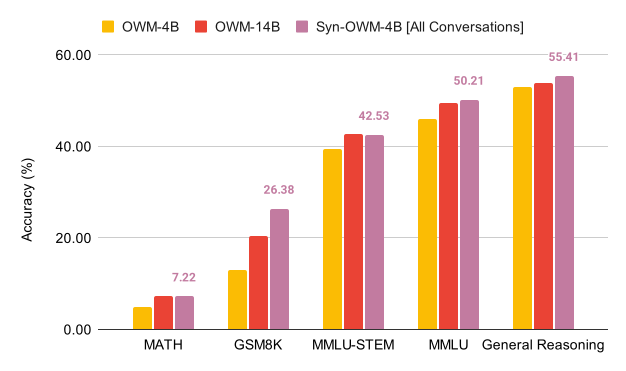
\includegraphics[trim={0 20 0 0}, clip, width=\textwidth]{figures/comp_data.pdf}
%     \caption{\label{fig:comp_data}}
% \end{wrapfigure}
\begin{comment}
In this work, we summarize the above observations in three key challenges associated with the generation and utilization of synthetic data for mathematical reasoning: (1) how to generate synthetic data to improve mathematical and logical reasoning ability when the underlying domain specific data is limited (2) how to engrave diversity in the generations and (3) how to ensure consistent improvement in math reasoning without hurting the performance of general purpose reasoning tasks. To address these challenges, we propose \textbf{\ourapproach}, a simple approach to generate \textbf{Conv}ersational Synthetic \textbf{Math} data at scale. In particular, we demonstrate that transforming raw web text into structured conversations using an off-the-shelf open-source \llm significantly enhances the mathematical and logical reasoning abilities of {\llm}s compared to relying on unstructured raw or rephrased web text. Additionally, relying on the web text to generate conversation provides us the flexibility to preserve diversity of the web corpora. Our approach generates conversations from a raw text by prompting an open-source \llm (\llama) on seven diverse conversational styles. 
\end{comment}

% \syeda{Add the numbers to the contributions}
\vspace{-2mm}
\begin{itemize}[leftmargin=*]
\itemsep0em
    \item We propose a novel approach, \ourapproach, to generate structured conversational synthetic data for math reasoning. Leveraging \ourapproach, we produce 64B tokens of synthetic data using 14B tokens from \owm corpus.
    % \item We have comprehensively experimented with different conversation styles by varying the roles of the participants for generating conversation and show a comparison between them. We provide this insight about the knowledge gap between two participants of a conversation to be a necessity in generating high quality math data.
    \item  We conduct comprehensive experiments with various conversational styles, altering participant roles to assess their impact on conversation quality and reasoning tasks. Our findings emphasize the importance of the knowledge imbalance between participants in producing high-quality mathematical data.
    % \item Additionally, we compare our approach with simple rephrasing of documents and chain of thought style of synthetic generation.
    \item We scale our approach to higher number of tokens and to two math specific datasets, demonstrating its efficacy in large and high-quality raw corpus.
    % \item Additionally, we provide insights into how the synthetic data and its combination with raw data should be provided during pretraining. \shrimai{Don't present the raw data as is. Rethink the data format.}
    \item %We demonstrate an effective way to integrate synthetic and raw data during pretraining that leads to a 6.29\% average improvement across three math benchmarks compared to raw data alone, emphasizing the importance of carefully reformatting raw data to optimize reasoning processes instead of using it in its original form.
    We demonstrate an effective way for integrating synthetic and raw data during pretraining to enhance mathematical reasoning ability of {\llm}s, emphasizing the importance of carefully reformatting raw data to optimize reasoning processes instead of using it in its original form. 
    % \item \shrimai{Check if we can release the data generated by llama 70B or 340B. Check if we can release the generation code and TRT-LLM pipeline.}
\end{itemize}
\vspace{-2mm}

% \shrimai{Improve this para, many confusing phrases.}
% In this paper, we evaluate \ourapproach across three dimensions: (1) the effectiveness of each conversational style in mathematical reasoning, (2) whether the impact of conversation persist as data scales, and (3) whether \ourapproach remains beneficial when the raw text originates from high-quality sources. When pretraining a 7B parameter \llm separately on a subset of \owm (\owma-4B) and synthetic conversations from \ourapproach (\ourdata-4B), the latter model achieves up to 6.29\% average improvement across three mathematical reasoning benchmarks, 4.30\% on specialized knowledge tasks (\mmlu), and a 2.20\% boost across 10 zero-shot tasks, compared to model trained with raw data. %In addition, our experiment using synthetic conversations on a single style generated from scaled raw data exhibits a consistent trend, demonstrating that conversational data enhances model performance even as datasets expand. 
In this paper, we evaluate \ourapproach across three dimensions: (1) the effectiveness of each conversational style in mathematical reasoning, (2) whether the impact of conversation persist as data scales, and (3) whether \ourapproach remains beneficial when the raw text originates from high-quality sources. Continuously pretraining a 7B \llm on synthetic conversations (\ourdata-4B), generated from a subset of \owm (\owma-4B), results in 6.29\% average improvement across three mathematical reasoning benchmarks, 4.30\% on specialized knowledge tasks (\mmlu), and a 2.20\% boost across 10 zero-shot tasks, compared to the model trained with raw \owma-4B. Additionally, our experiment with entire \owm (\owma-14B) and its corresponding synthetic conversations shows a consistent trend, indicating that the benefits of conversational data continue to hold as the data scales.
In fact, with all conversations generated from \owma-4B, we can outperform model trained with \owma-14B, a 3.6$\times$ larger data---2.94\% average improvement across \gsm and \mathall tasks, 1.56\% across all benchmarks (\autoref{fig:intro_img}). This underlines the value of synthetic conversations, particularly when high-quality in-domain data is limited. Moreover, our analysis with other datasets reveals that conversational data further amplifies reasoning capabilities in models even when the raw data originates from high-quality sources. We hope that \ourapproach will pave a way to improve complex reasoning ability of smaller models with limited training data and accelerate further innovation towards building strong reasoning ability with structured high-quality data.

%Ablations: (1) comparison with simple rephrasing (2) what is the best balance of raw and synthetic data (3) how to assess the quality of the generations. (4) ideal configuration for synthetic data generation


% This work aims to augment the reasoning ability of {\llm}s by generating conversational synthetic data that inherently requires deep comprehension of multi-hop scenarios and long context understanding. Our approach not only prepares a high-quality pretraining data for LLMs but also enhances the downstream reasoning tasks performance.
%Drawing the observation that complex problem solving benefits from step-by-step breakdown of the problem, we prompt 

% we introduce \ourapproach, a simple yet effective framework to generate synthetic mathematical data at scale for pretraining. In addition, solving complex reasoning problems such as math questions heavily benefits from breaking them down into smaller sub-problems step-by-step, enabling the model to process and tackle each component more effectively \citep{wei2022chain}.
 

%Additionally, synthetic data generation can introduce a significant ``knowledge bias" by selectively focusing on tasks that the model is intended to excel at. While synthetic data has demonstrated potential in improving performance \citep{rephrasing-the-web} during pretraining, it remains unclear whether this improvement stems from the inherently higher quality of synthetic data or from the deliberate choice of task-specific topics \citep{maini_phi_1_5}. 
    

%Yet they fall short when the underlying task demands complex and multi-hop logical reasoning specifically the mathematical reasoning tasks \citep{arora-etal-2023-llms, lu2023chameleon, he-etal-2024-olympiadbench, be83ab3e}.


% Distribution of high quality data sources is very skewed. Synthetic data can help create more balanced data sets.





% 1. We propose a novel synthetic data generation approach that goes beyond generating surface level linguistic variations and enhances raw text with semantic variations by adopting multi-hop conversational and reasoning format.
% 2. To promote diverse synthetic data generation at scale, this approach extends the synthesis across seven different conversational styles which steers the LLM towards the corresponding perspective to create distinctive synthetic data.
\section{\ourapproach: Math Informed syNthetic Dialogue Generation}

\begin{figure}[H]
  \centering
  \includegraphics[width=\columnwidth]{figures/method_eq_name.pdf}
  \caption{\textbf{Math Informed syNthetic Dialogue.} We (a) manually design prompts of various conversational styles, (b) provide the prompt along with raw context as input to \llm to obtain diverse synthetic conversations, (c) apply heuristic filtering to refine the generated data and (d) observe the downstream task performance after continuously pretraining an 7B \llm.}%\shrimai{why is there a snowflake in the ``conversational generator"? We should remove this. It looks like the snowflake company logo. The figure looks much better now. I am wondering if there is a way to indicate that MIND is the left part of the figure and we evaluate the utility of MIND by doing the right part of the figure. I don't see any reference to this figure in the text. Please refer to this figure when you are describing the mathematical formulation and later in 3.1 and 3.2}\syeda{just to clarify `snowflake' here represents frozen LLM}}
  \label{fig:conv_math}
\end{figure}

% \shrimai{The heading says \ourapproach: Pretraining with Conversational Synthetic Math Data whereas everywhere else we write that it is a `conversational synthetic data generation approach'. I think we should keep it consistent.}
%Generating high-quality synthetic mathematical data at scale using off-the-shelf \llm is challenging and expensive due to the in-feasibility of verifying the quality of large scale mathematical contexts. %Unlike the synthetic SFT corpora which are built focusing on specific downstream tasks, it is difficult ensure diversity and scalability when it comes to generating pretraining corpora. 
%To address the data diversity and generation cost problems
\vspace{-3mm}
To generate high-quality data at scale, current synthetic data generation approach explores rephrasing texts using {\llm}s in varied syntax while preserving the core content \citep{rephrasing-the-web}. %However, this type of rephrasing limits up-sampling high-quality data in a way that does not go beyond grammatical styles or surface form transformations. %In addition, this approach can not inject new knowledge such as complimentary reasoning or explanations to the context which is important for complex problem solving. 
% In addition
However, their proposed approach limits up-sampling high-quality data in a way that does not go beyond grammatical styles or surface form transformations---leading little to no improvement when it comes to performance across complex and logical reasoning tasks. %(e.g., HellaSwag \citep{zellers2019hellaswag}, Winogrande \citep{sakaguchi2019winogrande}, \mmlu \citep{hendryckstest2021} etc.). 
We hypothesize that simple rephrasing does not leverage the full potential of the synthetic data to improve the mathematical and complex multi-hop reasoning ability of \llm. Therefore, we propose, \textbf{\ourapproach}, a conversational synthetic data generation approach that adds semantic variations and structured complexity to the raw text which is required to improve complex reasoning ability of the {\llm}s. In addition, multi-turn conversations can break down the original context step-by-step while each step addresses a sub-context at a time by often injecting complimentary reasoning or explanations. This resonates with how human solves a complex problem using consecutive chain-of-thought reasoning.

As depicted in \autoref{fig:conv_math}, given a raw dataset $\mathcal{R}=\{r_1, ...r_N\}$, we define a set of conversational prompts $\mathcal{P}=\{p_1, ...p_7\}$ and utilize a pretrained \llm, denoted as $\mathcal{M}$, for synthetic data generation.  We combine raw data $r_j$ with a prompt 
$p_i$ and pass it to $\mathcal{M}$ to produce synthetic conversation $s_{i,j}$.
\[
    s_{i,j} = \mathcal{M}(p_i \, || \, r_j)
\]
Here, \(s_{i,j}\) represents the synthetic data generated by applying prompt \(p_i\) to the raw example \(r_j\). For a specific prompt, the total synthetic data generated can be represented as 
% \[\mathcal{S} = \{s_{i,j} \mid i \in [1, 7], j \in [1, N]\}\] 
\[
\mathcal{S} = \{s_{i,j} \mid j \in [1, N]\} \text{ for a fixed } i \in [1, 7]
\]
We further apply heuristic filtering ($\mathcal{H}$) to remove bad generations:
\[
   \mathcal{S}' = \mathcal{H}(\mathcal{S})
\]

Finally, we have a high-quality synthetic dialogue corpus $\mathcal{S}'$ which is specifically designed to improve mathematical and logical reasoning ability. To summarize \ourapproach:
\[
   \mathcal{R} \rightarrow \text{\ourapproach} \rightarrow \mathcal{S}'
\]
To evaluate the effectiveness of $\mathcal{S}'$ in pretraining, we conduct continuous pretraining on a base \llm, $\mathcal{C}$, to minimize the computational costs associated with full pretraining. Our prior experiments on complete pretraining with raw data, $\mathcal{R}$ and synthetic data, $\mathcal{S}'$ validates that the ranking between models trained on $\mathcal{S}'$ or $\mathcal{R}$ remains consistent whether we use continuous pretraining or full-scale pretraining (detailed in Appendix \ref{ss:pt_results}). Moreover, continuous pretraining has emerged as an effective way  to improve performance of {\llm}s in target domains \citep{guo2024efficient, huang2023lawyer, chen2023meditron} and even boost their general capabilities \citep{ibrahim2024simple, parmar2024reusedontretrainrecipe} with reduced training cost. Given the similar outcomes and significant savings in computational resources, we adopt continued pretraining for evaluating our approach throughout the paper.

Using $\mathcal{S}'$ and a subset of pretraining data ($\mathcal{R}_{pt}$), the model $\mathcal{C}$ is continuously pretrained, yielding an enhanced model $\mathcal{E}$, which possess improved mathematical reasoning capabilities.
\[
   \mathcal{E} \leftarrow \text{pretrain}(\mathcal{C}, \mathcal{D}); ~\text{where} ~ \mathcal{D} = \{\mathcal{S}' \cup \mathcal{R}_{pt}\}
\]


% \shrimai{We need to add more details here: (1) this is not part of MIND, this is done to evaluate how good $ \mathcal{S}'$ is, (2) Why we pick this setup of continuous training? to save cost and resources. pretraining is costly and we have our old results of pretraining. We can put them in appendix and write here that our preliminary expts had shown that ranking between different methods does not change if we do CT vs complete pretraining. Alternatively, you can also find some citation for this. Give intuition about this setup here.}

% \shrimai{Mathematical formulation of your problem and pipeline. Given a raw data $\mathcal{R}$, we have a set of conversational prompts $p=\{p_1, ...p_7\}$ and a pretrained LLM used for generation of synthetic data $\mathcal{M}$. We take prompt $p_1$  and raw data and we generate synthetic data $s_1$. (mapping of raw data, prompt, model used for generation and synthetic data that you get out it.). Then we use $s_1$ in continued training setup of another model $\mathcal{C}$. At the end of that continued training you get model $\mathcal{E}$.}

% In this section, we introduce the detailed methodology of \ourapproach, as depicted in \autoref{fig:conv_math}. We first outline the data synthesis approach (Section \ref{ss:data_synthesis}). Next, we describe the training configuration for validating the significance of the synthetic corpus (Section \ref{ss:training_config}).

% \subsection{Conversational Data Synthesis} \label{ss:data_synthesis}

% Our conversational data synthesis approach comprises of following steps:

\subsection{Compose Conversational Prompts} 
To generate conversation using a document $r_i$, we prompt $\mathcal{M}$ in a way that preserves all information from the original context in the conversation and remains faithful to the context. 
We manually compose several prompts on diverse conversation setting and topics. We finalize seven prompts ($\mathcal{P}$) featuring conversations between (1) \tss, (2) \ts, (3) \tp, (4) \deb, (5) \ps, (6) \lk, and (7) \intr which can be found in Appendix \ref{ss:prompts}. These prompts are specifically designed to guide \llm in breaking down the input context step-by-step, with each step being discussed in depth through explanations and reasoning. %As a result, unlike simple rephrasing, the conversations generated using these prompts highlight decomposition of complex contexts into smaller contexts and include varied perspective about a single context coming from different participants.

%The selection criteria for the prompts are that they instruct the \llm to break down the input context step-by-step and discuss each step comprehensively by adding explanations and reasoning to it. 

% compose seven different prompts to instruct the \llm: (1) Two Students, (2) Teacher Student, (3) Two Professors, (4) Debate, (5) Problem Solving, (6) Layman Know-All, and (7) Interview. The key feature of each prompt is that, () it instructs the \llm to break down the input context step-by-step and discuss each step comprehensively by adding explanations and reasoning to it.


\subsection{Generate Conversation} 
Given an unstructured raw text ($r_{j}$), we instruct the \llm to convert the raw text into a multi-turn conversation ($s_{i,j}$) using a prompt ($p_{i}$) where $p_{i} \in ~\{\text{two\_students}, \text{teacher\_student}, ..., \text{debate}\}$.
% \begin{equation}
%     C_{p_j} = \llm(p_j \, || \, t_i)
%     \label{eq:conv_gen}
% \end{equation}


\textbf{Seed Data Selection.} The benefit of \ourapproach will get amplified for raw texts that require step-by-step analysis and chain of thought reasoning---the key features of a math corpus. Therefore, we choose \owm \citep{paster2023openwebmath} as our seed corpus, $\mathcal{R}$, which contains 14.7B tokens of high quality mathematical web text. %Therefore, we utilize raw texts from \owm to generate synthetic conversations at scale. \shrimai{combine 2 sent}


% \textbf{Large Language Model.} We use \llama \citep{llama3modelcard} as the \llm to generate conversation from raw text. \llamabase is an an auto-regressive language model with an optimized transformer architecture. The instruction tuned model is finetuned and optimized for for dialogue/chat use cases. The major requirements for the conversation generator are (1) to ensure no information loss between raw text and conversation and (2) to remain grounded to the raw text. Unlike smaller {\llm}s, the generated conversation from \llama  remains grounded to raw text and expands on it by adding reasoning and explanation in each turn of conversation.

\textbf{Large Language Model.} We use $\mathcal{M}=~$\llama \citep{llama3modelcard} to generate conversations from raw text, due to its superior performance across a variety of tasks compared to other open-source models. 
%\llamabase is an auto-regressive language model built on an optimized transformer architecture. 
The instruction-tuned version is specifically fine-tuned and optimized for dialogue and chat-based applications. 
% \shrimai{edit here}
%The key requirements for the conversation generator are (1) to prevent any loss of information between the raw text and the conversation, and (2) to ensure the conversation remains faithful to the original text. 
%Unlike smaller {\llm}s, \llama generated conversations stay closely grounded in the raw text, expanding on it with reasoning and explanation in each conversation turn.


\textbf{Generation Configuration.} We observe that with increasing context length, conversations tend to lose details from the original texts, as discussed in Appendix \ref{ss:context_len}. Therefore, for each generation, we iteratively take contexts of 500 tokens to obtain accurate and informative conversations. To evaluate the quality of the generated conversations, we test various filtering methods, from simple heuristics to \llm-based scoring. However, as noted in Appendix \ref{ss:quality_assess}, \llm scoring consistently rates all generations highly, making it unsuitable for our approach. Hence, we rely on heuristic filtering to discard bad generations before using them for training.
%Further details on context length and quality assessment of the conversation can be found in Section \ref{ss:context_len} and \ref{ss:quality_assess}.  

\section{Experimental Setup}

% \subsection{Generation Details} \label{ss:generation_config}

\paragraph{Conversation Generator Configuration.} To generate conversation, we consider zero-shot prompting $\mathcal{M}$, where we only pass a basic prompt (Appendix \ref{ss:prompts}) and the raw text. We sample conversations with \texttt{temperature=1.0} and \texttt{top\_p=0.9} where the total number of input-output tokes is limited to 4096. We use the TensorRT-LLM toolkit to deploy large scale generation\footnote{\url{https://github.com/NVIDIA/TensorRT-LLM}}. 

% \subsection{Architecture}

\paragraph{Pretrained Model Architecture.} We train a standard decoder-only Transformer \citep{NIPS2017_3f5ee243} architecture of 7B parameters ($\mathcal{C}$). The framework uses causal attention masks and Rotary Position Embeddings (RoPE) \citep{su2021roformer},  Tiktoken tokenizer, SwiGLU \citep{shazeer2020gluvariantsimprovetransformer} activations in the MLP layers, and grouped query attention (GQA) \citep{ainslie-etal-2023-gqa}. The model consists of 32 layers, 32 attention heads, sequence length of 4096, and a hidden dimension size of 4096. It has no bias terms, has dropout rate of zero, and untied input-output embeddings. The models are trained using NVIDIA’s Megatron-LM \citep{shoeybi2019megatron} repository.


\subsection{Training Details}\label{ss:training_details}

\textbf{Pretraining Data.} Our pretraining data blend comprises of publicly available datasets from 13 snapshots of \cc (73.37\%) \citep{pile}, books/patents (9\%), papers (9\%), code (5.12\%), stack-exchange (2.66\%), and Wikipedia (0.8\%). Our code data consists of 42 programming languages while the other datasets come from various sources including web documents, news articles, scientific papers, and books. %We train the model on total 1T tokens of this data.

\textbf{General Pretraining.} To prepare a base model, we pretrain a 7B \llm on our pretraining data blend till 700B tokens using 512 H100 80GB SXM5 GPUs. During training, we use the AdamW optimizer \citep{loshchilov2018decoupled} with $\beta_1 =0.9$, $\beta_2=0.95$ and weight decay of 0.1. We use a 2-way tensor and pipeline parallelism to train the model. We set the maximum value of learning rate to $3e^{-4}$, minimum %learning rate 
to $3e^{-6}$, and use a batch size of 6M tokens with a 4096 context length.

% \shrimai{loss is pretraining loss.}

\textbf{Continued Pretraining.} After pretraining the base model ($\mathcal{C}$) on 700B tokens, we proceed with continuous pretraining using an additional 50B tokens to obtain $\mathcal{E}$. %\syeda{For our experiments, we create two baselines. The first baseline is formed by continuously training the base model on the pretraining blend till 50B tokens.} 
To reduce the shift between pretraining and continuous pretraining token distributions \citep{guo2024efficient} we %maintain consistency with the pretraining blend and 
create a new data blend ($\mathcal{D}$) for this phase.
To ensure the model is exposed to more math tokens, blend $\mathcal{D}$ consists of 2:1 ratio of \owm (33B tokens)---either raw ($\mathcal{R}$) or synthetic ($\mathcal{S}'$)--- and 13 snapshots of \cc (17B tokens) ($\mathcal{R}_{pt}$) to maintain consistency with the pretraining blend. %\shrimai{Aren't the same 13 CC used for pretraining upto 700B as well? Confirm and add the detail here}\syeda{No, I checked Dan's blend, the pretraining blend has all 13CC data with finewebedu score 0 to 5, here score 3,45 gets 1 epoch}. 
To ensure fair comparison, we always keep this token distribution constant in every experiment i.e., every model will see a the same amount of tokens from a data source regardless of its size. 
Unlike the pretraining blend, we use a high quality version of \cc data ($\mathcal{R}_{pt}$) filtered by the FineWebEdu \citep{penedo2024finewebdatasetsdecantingweb} classifier to achieve reasonable performance in generative tasks. This $\mathcal{R}_{pt}$ remains constant across all our continued pretraining experiments, while we vary the \owm %component by introducing synthetic data 
with $\mathcal{R}$ or $\mathcal{S}'$ or combining both to assess their relative significance. We maintain the same training configuration as before and continue pretraining until reaching 50B tokens, using the same pretraining loss objective. In this paper, we use two versions of \owm: 
\begin{itemize}[leftmargin=*]
\itemsep0em
\vspace{-2mm}
    \item \textbf{\owma-4B:} To quickly evaluate the effectiveness of all seven prompts, we take a smaller subset of \owm containing 4B tokens. Synthetic data generated from this subset is labeled as \ourdata-4B throughout the paper.
    \item \textbf{\owma-14B}: This version contains the full 14.7B tokens of \owm and the synthetic data of this is called \ourdata-14B.
\end{itemize}

\subsection{Evaluation Metrics}
% \subsection{Decay Experiments with data from 7 Conversational Styles}
To evaluate the zero-shot and few-shot learning capabilities of our models, we conduct a thorough benchmark assessment using a series of datasets using LM Eval Harness \citep{eval-harness}.

\textbf{General Purpose Reasoning Tasks.} This category comprises datasets testing broader cognitive skills and language comprehension. We consider nine standard commonsense and logical reasoning tasks in 0-shot: ARC easy (ARC-E) \& challenge (ARC-C) \citep{clark2018thinksolvedquestionanswering}, PIQA \citep{bisk2020piqa}, SIQA \citep{sap-etal-2019-social}, HellaSwag \citep{zellers2019hellaswag}, WinoGrande \citep{sakaguchi2021winogrande}, OpenBookQA \citep{OpenBookQA2018}, TruthfulQA \citep{lin-etal-2022-truthfulqa}, CommonsenseQA \citep{talmor-etal-2019-commonsenseqa} %. We further test the understanding and reasoning skills of the pretrained models on 
and a reading comprehension task: RACE \citep{lai-etal-2017-race}. We report the average results across ten general reasoning tasks under the metric `\textsc{General Reasoning}'.

\textbf{Math and Specialized Knowledge Tasks.} We consider three diverse math benchmarks to comprehensively evaluate the mathematical reasoning ability.
%using few-shot chain-of-thought prompting \citep{wei2022chain}. 
These benchmarks encompass mathematical challenges from elementary to college level complexity demanding qualitative reasoning (8-shot \gsm \citep{cobbe2021training}, 4-shot \mathall \citep{hendrycksmath2021}) and conceptual science and math reasoning %in multiple-choice question format 
(5-shot \mmlus \citep{hendryckstest2021}). In the Specialized Knowledge category, we evaluate on % include dataset that demand expertise in specific domains. 
\mmlu that spans multiple domains, from professional to academic, testing the model on specialized subjects.


% To quickly evaluate the effectiveness of different prompts, we begin with a subset of \owm containing 4B tokens, which we label as \owma-4B. The synthetic data generated from this subset is referred to as Syn-\owma-4B. For experiments involving the full 14.7B tokens of \owm, we label it as \owma, with the corresponding synthetic data termed Syn-\owma. 



% \subsection{}






\input{sections/experiments_revision}
\section{Ablations}\label{sec:ablations}

% In this section, we will analyze the significance of prompt style (Section \ref{ss:prompt_effect}), effect of conversation on other datasets (Section \ref{ss:other_data}), the efficient way to utilize synthetic data (Section \ref{ss:data_prep}), and comparison with other synthetic data generation approach (Section \ref{ss:comp_rephrase}). We will also discuss the effect of input context length for conversation generation (Section \ref{ss:context_len}) and navigate ways to assess the quality of the conversation (Section \ref{ss:quality_assess}).

% In this section, we analyze the significance of prompt styles, scalability on  other datasets, the efficient way to utilize synthetic data, and comparison with other synthetic data generation approach. We also discuss the effect of input context length for conversation generation (Appendix \ref{ss:context_len}) and navigate ways to assess the quality of the conversation (Appendix \ref{ss:quality_assess}).

% \shrimai{Points to make
% \begin{itemize}
%     \item Show that conversational styles are comparable to original OWM
%     \item show that conversational styles are better than rephrase and CoT
% \end{itemize}}

% \subsection{Does the Prompt Style matter?}
% We measure the 

% \subsection{Does the Prompt Style matter?}\label{ss:prompt_effect}


\paragraph{Does the Prompt Style matter?} \label{ss:prompt_effect}
%To evaluate the impact of prompt styles, we conduct experiment by training with conversations from seven different styles. 
From \autoref{tab:7b_owm_4b}, we observe improvement across all tasks using six conversational styles. However, our experiment with \tp conversations yield relatively equivalent or worse performance compared to the raw data (\autoref{tab:7b_tp}). 



\begin{table*}[h!]
\begin{center}
\resizebox{\textwidth}{!}{% 
\begin{tabular}{@{}lccccccc@{}}
\toprule
\textbf{Dataset} & \textbf{Style} & \textbf{GSM8K} & \textbf{MATH}	& \textbf{\shortstack{MMLU-\\STEM}} & \textbf{\shortstack{MMLU}} & \textbf{\shortstack{\textsc{General Reasoning}\\(Avg)}}&\textbf{Avg-All}\\\toprule
\owma-4B &   Raw & 12.96	&4.92	&39.39	&45.91	&52.90&29.17\\ \midrule
% & \mawps           & \textbf{69.83}         & 66.83            \\ 
\ourdata-4B & \tp & 13.50	&4.52	&37.93	&45.25	&53.21&29.12\\
\toprule
\end{tabular}
}
\end{center}
\vspace{-2mm}
\caption{\textbf{\tp prompt style vs Raw data.} Continuous pretraining with \tp conversations does not provide gain over raw data compared to other conversational styles.}
\label{tab:7b_tp}
\end{table*}


% This outcome can be attributed to the nature of the \tp conversation style. Upon reviewing the generated conversations, we hypothesize that the relatively lower performance is due to the surface-level engagement between the two professors. In this setup, both participants assume that the other already has sufficient knowledge as they are the domain experts, leading to less detailed discussions. This contrasts with other styles where there is either a clear knowledge gap between participants (\lk, \ts, \intr) or both participants being non-experts are actively analyzing and solving the problem (\ps, \deb, \tss), forcing participants to explain concepts in more depth, which results in expanded dialogues with complementary explanations and reasoning.

\begin{wrapfigure}[14]{r}{0.5\textwidth}
    \vspace{-6mm}
    \centering    
    \includegraphics[trim=0 20 0 0, clip, width=\textwidth]{figures/bleu_rogue.pdf}
    \caption{\textbf{Similarity between Raw Text \& Synthetic Dialogues.} The \tp style exhibits greater similarity to raw text, while \lk shows the lowest similarity due to its richer context with details and explanations.} 
    \label{fig:bleu_rouge}
     \vspace{-1mm}
\end{wrapfigure}

This outcome can be attributed to the nature of the \tp conversation style. 
Upon reviewing the generated conversations, we hypothesize that the relatively lower performance is due to the zero-knowledge gap between participants. In this setup, both participants assume that the other already has sufficient knowledge as they are the domain experts, leading to surface-level engagement and less detailed discussions.

To further investigate, we measure the BLEU and ROUGE scores between the raw text and the corresponding conversation, as shown in \autoref{fig:bleu_rouge}, and find that the \tp style exhibits the highest similarity to raw text. This implies that \tp dialogues do not fully exploit the potential of the generation model to introduce new reasoning or breakdowns of complex problems, aligning with our qualitative observation that the professors are not engaging in deeper analysis of concepts. This contrasts with other conversational styles where there is either a clear knowledge gap between participants (\lk, \ts, \intr), forcing one to explain concepts in more depth, or both participants, being non-experts are actively analyzing and solving the problem (\ps, \deb, \tss) which results in expanded dialogues with complementary explanations and reasoning. In the latter case, the lack of expertise creates an implicit knowledge gap---instead of one participant being more knowledgeable, both non-experts collaborate to bridge their shared knowledge gap. As depicted in \autoref{fig:bleu_rouge}, the \lk style, which features the greatest knowledge imbalance between participants, has the lowest BLEU and ROUGE scores. This supports our hypothesis that a larger information gap encourages the knowledgeable participant to explain concepts thoroughly, leading to more explicit and detailed conversations. 

% We further analyzed the BLEU and ROUGE scores for all conversation styles, as shown in \autoref{fig:bleu_rouge}, and found that the \tp style exhibits the highest similarity to raw text. This suggests that \tp conversations do not fully exploit the potential of the generation model to introduce new reasoning or breakdowns of complex problems, aligning with our qualitative observation that the professors are not engaging in deeper analysis of concepts. In contrast, the \lk style, which features the greatest knowledge imbalance between participants, has the lowest BLEU and ROUGE scores. This supports our hypothesis that a larger information gap encourages the knowledgeable participant to explain concepts thoroughly, leading to more explicit, and detailed conversations. 

Relating these insights to our findings in \autoref{tab:7b_owm_4b}, we see that incorporating explicit knowledge gaps in dialogues is beneficial for \mmlu and general reasoning tasks. Conversely, collaborative problem solving, to close the implicit knowledge gap, %—where participants engage in reasoning together, often debating or complementing one another's ideas—
is crucial for improving performance on math tasks. This highlights a key characteristic of high-quality math data---merely breaking down the problem is insufficient for effective math reasoning. Instead, dynamic knowledge exchange and analysis within the dialogues are essential to achieve maximum improvement in math reasoning.

% Moreover, incorporating knowledge gap in dialogues is particularly beneficial for \mmlu and general reasoning tasks (\autoref{tab:7b_owm_4b}). In contrast, collaborating problem solving, where participants jointly deconstruct and analyze the problem, is advantageous for improving performance on math tasks.



% In this case, the knowledge gap encourages the knowledgeable participant to explain concepts thoroughly, which enhances the quality of the generated synthetic data and, subsequently, the model's reasoning ability.



% \subsection{Does Conversation benefit other datasets?}\label{ss:other_data}


\paragraph{Does Conversation benefit other datasets?} \label{ss:other_data}
% Our experiments so far have utilized \owm as the seed corpus for generating synthetic conversations and training  \llm. \owm is predominantly a mathematical corpus collected from mathematical web pages that can contain noisy web contexts. Generating synthetic conversations for such noisy contexts upsamples high-quality data and hence we observe a huge gain in performance with high-quality conversations. However, it is yet to be explored whether \ourapproach will work on high-quality datasets such as books or papers. To investigate this, we consider a new seed corpus, \mathpile \citep{wang2023mathpile}, that consists of 9.3B tokens extracted from high-quality data sources such as ArXiv papers, textbooks, StackExchange, Wikipedia, ProofWiki, and \cc pages.

\owm used in our current experiments is predominantly collected from mathematical web pages that can contain noisy web contexts. Generating synthetic conversations for such noisy contexts upsamples high-quality data and hence we observe a huge gain in performance with high-quality conversations. Here, we investigate if \ourapproach works on high-quality datasets such as books or papers. We consider a new seed corpus, \mathpile \citep{wang2023mathpile}, that consists of 9.3B tokens extracted from high-quality data sources such as ArXiv papers, textbooks, StackExchange, Wikipedia, ProofWiki, and \cc pages.

\begin{table*}[ht!]
\begin{center}
\resizebox{\textwidth}{!}{% 
\begin{tabular}{@{}lccccccc@{}}
\toprule
\textbf{Dataset} & \textbf{Style} & \textbf{GSM8K} &\textbf{MATH} & \textbf{\shortstack{MMLU-\\STEM}} & \textbf{MMLU}& 	\textbf{\shortstack{\textsc{General Reasoning}\\(Avg)}} & \textbf{Avg-All}\\\toprule
Pretraining Data & \multirow{2}{*}{Raw} & 9.33	& 4.74	& 37.84	& 45.41	& 53.22 & 28.17\\ 
\mathpile & & 8.79	&4.96	&	42.82 &49.49	&54.16	&29.35\\\midrule
\textsc{mind}-\mathpile & \tss & 12.74&	5.74	&43.55&	49.91	&53.98	&\textbf{30.59}\\ 
\toprule
\end{tabular}
}
\end{center}
\caption{\textbf{\mathpile vs Synthetic Conversation from \mathpile (\textsc{mind}-\mathpile).} Conversation generated from high-quality raw data further improves the performance of math tasks.}
\label{fig:mp_exp}
\vspace{-2mm}
\end{table*}

By employing $\mathcal{M}$, we generate conversations from raw text with the \tss prompt. Later, we replicate the experiments %with \owma-4B and \ourdata-4B 
by replacing \owma with \mathpile and \textsc{mind}-\mathpile accordingly. \autoref{fig:mp_exp} shows that \textsc{mind}-\mathpile outperforms the raw counterpart in all three math benchmarks along with specialized knowledge tasks, achieving comparable scores in general reasoning task. 
In addition, majority of \mathpile data is from ArXiV papers and recent work has found this source ineffective in improving mathematical reasoning \citep{deepseek-math}. 
We observe a similar trend, where non-math focused pretraining corpora yields better \gsm score than raw \mathpile corpus. However, our synthetic conversation on \mathpile rather amplifies the quality of the corpus resulting in 3.95\% %and 2.96\% 
absolute improvement on \gsm in comparison with raw data. %and pretraining blend respectively. 
This highlights the superior structured complexity of conversations, which proves particularly effective for multi-hop and mathematical reasoning tasks, over high-quality data from Arxiv papers.% \shrimai{why the claim of high quality books? You only mention Arxiv in the para. Make it concrete and only talk about Arxiv.}.

% \begin{figure}[H]
%   \centering
%   \includesvg[width=0.8\columnwidth]{figures/mathpile.svg}
%   \caption{\textbf{\mathpile vs Synthetic Conversation from \mathpile (Syn-\mathpile).} Conversation improves the performance of math tasks even when the raw data derives from high-quality sources.}
%   \label{fig:mp_exp}
% \end{figure}



% \subsection{Rephrase vs Conversation}\label{ss:comp_rephrase}

% \paragraph{Rephrase vs Conversation.}\label{ss:comp_rephrase}


% \begin{table*}[ht!]
% \begin{center}
% \resizebox{\textwidth}{!}{% 
% \begin{tabular}{@{}lccccccc@{}}
% \toprule
% \textbf{Dataset} & \textbf{GSM8K} &\textbf{MATH} & \textbf{\shortstack{MMLU-\\STEM}} & \textbf{MMLU}& 	\textbf{\shortstack{\textsc{General Reasoning}\\(Avg)}} & \textbf{Avg-All}\\\toprule
% % Pretraining Data & 9.33	& 4.74	& 37.84	& 45.41	& 53.22 & 28.29\\ 
% \owma-4B  & 12.96	&4.92	&39.39	&45.91	&52.90&29.17\\\midrule
% Rephrase-\owma-4B  & 11.68 & 5.46 & 39.71 & 46.17 & 53.58 & 29.22\\\midrule
% % \owma-4B+Rephrase-\owma-4B [1:1] & 14.25	&6.20	&42.31	&48.74	&53.68&	30.72\\\midrule
% \ourdata-4B [Longest Conversation]&  25.78 & 6.30 & 42.72 & 49.37 & 54.86 & 34.08\\

% % \owma-4B+\ourdata-4B [1:1]& & 21.68	&6.14	&42.56	&49.57	&54.50	&32.97\\
% \toprule
% \end{tabular}
% }
% \end{center}
% \caption{\textbf{Rephrase vs Conversations.} Continuous training of 7B \llm shows that conversational data is better for mathematical and general reasoning than simple rephrasing.}
% \label{tab:rephrase}
% \vspace{-2mm}
% \end{table*}

% %\shrimai{You don't say anything about the OwM + Rephrase case. If this result does not add any value then remove it. You can potentially add it to the next ablation ... and say that raw+syn makes most sense for rephrase case }\syeda{Passed it to the next section}
% As illustrated in \autoref{tab:rephrase}, model pretrained on conversations consistently outperforms those trained on rephrased or raw text across all tasks. %Although combining rephrase with raw text is better than only rephrased data, it still underperforms the model trained with conversations in math reasoning. 
% Interestingly, rephrased data underperforms raw data in benchmarks such as \gsm. This disparity is closely related to the limitations of the rephrasing process. Rephrase adds linguistic variations to the older data, preserving the syntactic meaning of the document, but can not generate semantic/pragmatic variations. Moreover, rephrases are limited to the information in the raw text and unable to inject new knowledge into the data. 
% %Conversational data, by contrast, provides a more dynamic framework. Conversations not only preserve the core information of the context but also enhance it through the interaction of participants, who can introduce different perspectives, ask clarifying questions, and elaborate on reasoning. This allows for the injection of new knowledge in the form of complementary explanations, deeper reasoning, and iterative problem-solving—all crucial components for solving complex reasoning tasks (Appendix \ref{ss:conv_example}). 
% As evidenced in our experiments, while rephrasing offers some benefits, it falls short in addressing the deeper, more complex reasoning challenges that conversational data can resolve. The structured and interactive nature of conversations facilitates a more nuanced understanding of the problem space, making it an effective approach for improving mathematical reasoning of {\llm}s.

% In contrast, conversation can enhance existing context with the perspective and conscience of participants who are discussing about the context. In addition, conversation creates space to inject knowledge in a form of complimentary explanations and reasonings in turns which are essential elements for solving complex reasoning problems (\syeda{add conversation examples}). 


% \subsection{Is replacing with Synthetic Data the best option?}\label{ss:data_prep}

\vspace{-1mm}
\paragraph{Is replacing with Synthetic Data the best option?}\label{ss:data_prep}
Our findings in \autoref{tab:7b_owm_4b}, \ref{tab:7b_owm} indicate that completely replacing \owm with synthetic data yields the best performance across benchmarks. However, %prior work 
\cite{rephrasing-the-web} emphasizes the importance of combining real data and synthetic rephrases to achieve consistent improvements across a broader range of tasks---a similar trend we observe in our experiment with rephrased data, as shown in \autoref{tab:7b_comp_data}. To investigate this further, we conduct experiments with four data combinations using \owma-4B while the $\mathcal{R}_{pt}$ remains constant:

\begin{itemize}[leftmargin=*] 
\itemsep0em
% \vspace{-1mm}
\item \textbf{\owma-4B + \ourdata-4B [1:1].} We combine $\mathcal{R}$ and $\mathcal{S}'$ in a 1:1 ratio, ensuring an equal number of tokens to be seen during pretraining from both sources. For the synthetic data, we utilize the \textsc{Longest Conversation}, as this shows the most improvement across tasks (\autoref{tab:7b_owm_4b}). 
\item \textbf{\owma-4B + \ourdata-4B [Concat].} We concatenate each raw context with all seven synthetic conversations sequentially. 
\item \textbf{\ourdata-4B [Longest Conversation].} From the seven conversations generated for each context, we select the longest conversation in token count. 
\item \textbf{\ourdata-4B [All Conversations].} This data incorporates all conversation across all styles. 
\end{itemize}






\begin{table*}[h!]
\begin{center}
\resizebox{\textwidth}{!}{% 
\begin{tabular}{@{}lcccccc@{}}
\toprule
\textbf{Dataset} & \textbf{\gsm} &\textbf{\mathall} & \textbf{\shortstack{\mmlus}} & \textbf{\mmlu}& 	\textbf{\shortstack{\textsc{General Reasoning}\\(Avg)}}&\textbf{Avg-All}\\\toprule
\owma-4B & 12.96	& 4.92	& 39.39	& 45.91	& 52.90&29.17\\ 
\owma-14B & 20.47 & 7.24 & 42.82 & 49.49 & 53.95& 32.79\\\midrule
Rephrase-\owma-4B  & 11.68 & 5.46 & 39.71 & 46.17 & 53.58 & 29.22\\
\owma-4B+Rephrase-\owma-4B [1:1] & 14.25	&6.20	&42.31	&48.74	&53.68&	30.72\\\midrule
\owma-4B+\ourdata-4B [1:1] & 21.68 & 6.14 & 42.56 & 49.57 & 54.50&32.97\\ 
\owma-4B+\ourdata-4B [Concat] & 24.49 & 6.22 & \textbf{43.67} & \textbf{50.46} & 55.10&34.07\\
\ourdata-4B [Longest Conversation] & 25.78 &	6.30 & 42.72 & 49.37 & 54.86&34.08\\ 
\ourdata-4B [All Conversations] & \textbf{26.38} & \textbf{7.22} & 42.53 & 50.21 & \textbf{55.41}&\textbf{34.80}\\ 
\toprule
\end{tabular}
}
\end{center}
\caption{\textbf{Comparison of 7B \llm trained with raw and combination of synthetic data.} Synthetic conversation outperforms raw data in all combinations. Specifically, combinations of all conversations generated from \owma-4B surpasses the performance of \owma-14B (3.6$\times$ larger corpus) across all tasks, underscoring the superior quality and diversity of the conversations.}
\label{tab:7b_comp_data}
\vspace{-2mm}
\end{table*}

Our finding in \autoref{tab:7b_comp_data} indicates that all combinations provide substantial boost in performance across all tasks. However, for math-centric benchmarks (\gsm and \mathall), training solely with synthetic conversations elicits the best improvements. This is likely as these tasks require complex and multi-step reasoning and conversations are designed to replicate these type of thinking. In parallel, having both raw data and conversation is beneficial for specialized and general purpose reasoning tasks, aligning with the findings in \cite{rephrasing-the-web}. Since synthetic data tends to remove special tags, styles, and code indentations, the inclusion of raw data helps improve the generalizability of {\llm}s across diverse domains. Additionally, to measure the maximum gain we can achieve from conversations for a limited data, we %run another experiment with all synthetic conversations generated from \owma-4B. 
continuously train $\mathcal{C}$ with all synthetic dialogues generated from \owma-4B.  %Consistent with previous experiments, we kept the input token count constant during training. 
As shown in \autoref{tab:7b_comp_data}, using conversations generated from \owma-4B, we can outperform the model trained with 3.6$\times$ bigger corpus (\owma-14B) on \gsm, \mmlu and general reasoning tasks while showing comparable performance on other tasks. Inspired by this, we further compare \ourapproach with \dsm \citep{deepseek-math} that extract 120B unique math tokens from \cc (Appendix \ref{ss:dsm}). The results from \autoref{tab:dsm_exp} demonstrate that diverse conversations from \ourapproach based on a small seed corpus can yield comparable math accuracy to the \dsm model. This illustrates the potential to enhance reasoning with limited data by generating synthetic conversations of infinite styles.

% \begin{figure}[H]
%   \centering
%   \includesvg[width=0.8\columnwidth]{figures/PT_comparison.svg}
%   \caption{Training with only synthetic data yields the best results for MMLU.}
% \end{figure}

\paragraph{Does the improvement persist with smaller $\mathcal{M}$?} In the previous experiments, we used a constant $\mathcal{M}$, a powerful instruction-tuned model. However, it remains unclear whether the improvements in downstream reasoning tasks stem from the quality of the generated dialogues or are primarily due to model distillation from the powerful \llm. To asses the impact of $\mathcal{M}$ on the downstream task performance, we re-run \ourapproach with a smaller $\mathcal{M}$=\llamas on \ps style, the best performing style in \autoref{tab:7b_owm_4b} and continuously pretrained a 7B \llm following the training setup in Section \ref{ss:training_details}.

\begin{table*}[h!]
\begin{center}
\resizebox{\textwidth}{!}{% 
\begin{tabular}{@{}lccccccc@{}}
\toprule
\textbf{Dataset} & \textbf{$\mathcal{M}$} & \textbf{GSM8K} &\textbf{MATH} & \textbf{\shortstack{MMLU-\\STEM}} & \textbf{MMLU}& 	\textbf{\shortstack{\textsc{General Reasoning}\\(Avg)}} & \textbf{Avg-All}\\\toprule
\owma-4B & - & 12.96	&4.92	&39.39	&45.91	&52.90&29.17\\\midrule
\multirow{2}{*}{\ourdata-4B} & \llamas & 22.37	&5.72&	41.36&	48.48 & 55.21 &32.95\\
& \llama & 24.72 & 6.16	& 41.36	& 47.74 & 54.90 & 33.38\\
\toprule
\end{tabular}
}
\end{center}
\caption{\textbf{Results of 7B \llm trained on \ourdata-4B using $\mathcal{M}$ of different sizes:} Regardless of the sizes of $\mathcal{M}$, model trained on \ourdata-4B outperforms the one trained with raw data.}
\label{tab:diff_m}
\vspace{-2mm}
\end{table*}

As shown in \autoref{tab:diff_m}, even with a smaller $\mathcal{M}$, the \ourapproach-generated data provides a significant boost in math and general reasoning abilities compared to the raw/rephrased data. This demonstrates that the gains are not solely dependent on the capabilities of the larger $\mathcal{M}$ but are largely driven by the quality and structure of the MIND-generated dialogues. Additionally, regardless of model size and method of synthetic data generation, all \llm-generated synthetic data involves some form of knowledge distillation. However, we demonstrate an effective distillation approach that significantly enhances the reasoning ability of {\llm}s compared to existing approaches \citep{rephrasing-the-web}.

\vspace{-2mm}


% % \subsection{Context Length vs Conversation Quality}\label{ss:context_len}



% \paragraph{Context Length vs Conversation Quality.}\label{ss:context_len}
% To generate conversations, we utilize $\mathcal{M}$, which supports input sequences of up to 8K tokens. However, the \owm corpus, composed of mathematical web pages from Common Crawl, often contains documents exceeding this 8K token limit, leading to errors when processing them with the \llm. A straightforward approach is to split these inputs into 8K-token windows, but initial experiments with this method reveal significant drawbacks. Conversations generated from the 8K-token inputs tend to summarize the lengthy context, resulting in a loss of substantial information from the original text. 

% \begin{wrapfigure}[11]{r}{0.45\textwidth}
%     \vspace{-6mm}
%     \centering    
%     \includesvg[width=\textwidth]{figures/context_len.svg}
%     \caption{With increasing context length the generated conversation length decreases.} 
%     \label{fig:context_length}
% \end{wrapfigure}
% Therefore, we conduct an experiment on 140k samples from the \owm corpus of varying input length to determine the optimal input token length that generates conversations of following characteristics: (1) retains all relevant information from the original context, (2) remains grounded to the source material and (3) enhances the conversation with complementary explanations and reasoning. For each sample, we generate conversations using two prompt (\tp and \ts) and observe the token length of the generations. As depicted in \autoref{fig:context_length}, with increasing input token length (X-axis), the token length of the generated conversation (Y-axis) does not scale up linearly. For example, an input context of 2K tokens results in a conversation that has 1K tokens resulting in a lot of information loss during conversion. Analyzing the \autoref{fig:context_length}, we see that the input token length of 500 can generate conversation that goes beyond 500 tokens meaning that the conversation not only retains information but also adds necessary reasoning  resulting in more tokens. 

% % \begin{figure}[H]
% %   \centering
% %   \includesvg[width=0.8\columnwidth]{figures/context_len.svg}
% %   \caption{With increasing context length the generated conversation length decreases!}
% %   \label{fig:context_length}
% % \end{figure}




% % \subsection{Conversation Quality Assessment}\label{ss:quality_assess}

% \begin{wrapfigure}[13]{r}{0.45\textwidth}
%     \vspace{-6mm}
%     \centering    
%     \includesvg[width=\textwidth]{figures/quality.svg}
%     \caption{LLM tends to rate its generation higher most of the times.}
%   \label{fig:conv_quality}
%   \vspace{-2mm}
% \end{wrapfigure}
% \paragraph{Conversation Quality Assessment.} \label{ss:quality_assess}
% While the conversations generated by the \llm typically appear coherent, there are instances where the output fails to preserve the context or lacks grounding to the source material. In some cases, conversations may even be incomplete. Detecting poor-quality generation becomes challenging at scale. To address this, we explore two quality-filtering approaches:

% \textbf{Heuristic Filtering.} We employ a simple heuristic based on token length. Given that the input context is limited to a maximum of 500 tokens and split into subcontexts of 500 tokens each to maximize information retention, we discard any generated conversations that fall below 50 tokens. This ensures that minimal information loss is detected early.

% \textbf{\llm-based Scoring.} For a more comprehensive assessment, we use an \llm to score the quality of the generated conversations. We introduce four key metrics for evaluation:
% \begin{itemize}[leftmargin=*] 
%     \item \textbf{Correctness}: Verifies that all information, such as numbers and parameters, is accurately reflected in the conversation.
%     \item \textbf{Faithfulness}: Ensures the conversation remains grounded in the context provided.
%     \item \textbf{Information Preservation}: Checks whether all relevant facts and knowledge from the original context are retained in the conversation.
%     \item \textbf{New Knowledge}: Evaluates whether the conversation introduces additional explanations, reasoning, or definitions not present in the raw input.
% \end{itemize}

% Given a raw context and its corresponding conversation, we ask $\mathcal{M}$ to rate the conversation on a scale of 1 to 5 in each of four metrics, with 1 representing poor quality and 5 representing the best possible conversation. To determine the overall quality, we compute the average score across the metrics and choose conversations with average scores more than or equal to 3. Additionally, we utilize the prompt from the FineWebEdu \citep{penedo2024finewebdatasetsdecantingweb} annotation framework to further check the correlation between two scoring approaches. In \autoref{fig:conv_quality}, we plot the scores for 140K conversations using FineWebEdu metrics and our metrics. It is clearly visible from the figure is that \llm tends to rate its own generation higher almost all the time resulting in a skewed distribution of rating. Around 96\% of conversations are labelled as high quality. % comparison between fineweb metrics and our. our is better

% To further investigate, we choose 20 contexts and their corresponding conversations and manually label them on the above four metrics. We later pass these samples to \llm to obtain the quality scores. When comparing the human scores with those from the \llm, we noted discrepancies in both the scores and the reasoning behind them. Human annotators prioritized the information preservation metric, while the \llm often overlooked minor information loss. Additionally, the interpretation of ``New Knowledge" differed between humans and the \llm. Humans valued extra reasoning and explanation as forms of new knowledge, whereas the \llm assigned higher ``New Knowledge" scores to conversations containing out-of-context information that is difficult to verify. Given these differences in the results from human and \llm-based quality filtering, we use simple heuristic filtering in this study and plan to explore other approaches in the future.


% \begin{figure}[H]
%   \centering
%   \includesvg[width=0.8\columnwidth]{figures/quality.svg}
%   \caption{With increasing context length the generated conversation length decreases!}
%   \label{fig:conv_quality}
% \end{figure}





% * DSM multilingual chinese model - > improvements span over english and chinese tasks, so not very comparable
% * our internal result we get with their best model is worst than their published numbers, but evaluation pipeline is static
% * generation bug with the code tasks




\section{Related Works}

% \shrimai{We can move this section to before Conclusion}
\textbf{Mathematical Data Curation.} Selecting high quality data for pretraining {\llm}s is essential for producing state-of-the-art large language models \citep{NEURIPS2020_1457c0d6, chowdhery2023palm, parmar2024data, parmar2024nemotron, rae2021scaling, feng2024maximize}. Several mathematical datasets have been introduced in recent years \citep{paster2023openwebmath, wang2023mathpile, azerbayev2023proofnet, welleck2021naturalproofs} which have been carefully collected from the web using different heuristics. \owm contains 14.7B tokens of mathematical web pages filtered from \cc based on math strings, \LaTeX contents and a math document classifier. Building on this corpus, \dsm \citep{deepseek-math} trains a fastText \citep{joulin2016fasttext} classifier to further extract mathematical documents from \cc. They cluster the extracted documents based on the URL domain and label a domain math-related where over 10\% of the web pages have been collected are classified as math content. Finally, web pages linked to these URLs, yet uncollected, will be added to the seed corpus which will be used to retrain the fastText classifier to fetch diverse math contexts. \mathpile \citep{wang2023mathpile}, a multi-source corpus (8.9B tokens), has been aggregated from textbooks, Wikipedia, ProofWiki, \cc, StackExchange, and arXiv, with the majority (over 85\%) sourced from high quality data source arXiv. Although these datasets can effectively capture the diverse mathematical information from web, it is difficult to detect and filter out noisy dataset.
%and hence lowering the chances to obtain maximum gain from these corpora. 
Recently, many powerful models %, such as GPT-4 \citep{openai2024gpt4technicalreport}, Mistral \citep{jiang2023mistral7b}, Gemini \citep{geminiteam2024geminifamilyhighlycapable}, Claude \citep{anthropic}, Qwen \citep{qwen2.5} etc.
\citep{openai2024gpt4technicalreport, jiang2023mistral7b, geminiteam2024geminifamilyhighlycapable, anthropic, qwen2.5}, in addition to not open sourcing their data, are also refraining from disclosing detailed information about their corpus. % in their technical reports. 
For the open-source community, constructing high-quality and diverse pretraining corpora is a crucial factor in bridging the performance gap with closed-source models which is the main objective of our work. 

\textbf{Synthetic Math Data.}  Generating synthetic math data using {\llm}s has been widely explored in recent days \citep{53097, li2024common7blanguagemodels, gunasekar2023textbooksneed, madaan2024self, patel-etal-2024-datadreamer, toshniwal2024openmathinstruct118millionmath} specifically during alignment using supervised fine-tuning (SFT) \citep{alpaca}.  Some of the latest approaches focus on generating data from seed problems. For instance, \cite{yu2023metamath} rewrites existing benchmark questions from multiple perspectives using {\llm}s to create new mathematical problems, while \cite{huang2024keypointdrivendatasynthesisenhancement, shah2024aiassistedgenerationdifficultmath} leverage \gptllm to extract topics and key points from seed samples and recombine them into new questions. %\cite{shah2024aiassistedgenerationdifficultmath} follows a similar approach to create more challenging and diverse mathematical evaluation set. 
To further improve diversity, \cite{chan2024scalingsyntheticdatacreation} uses \gptllm to generate questions and answers at scale, incorporating over one million personas. %to ensure variety in the output. 
Previous approaches to generate synthetic data is primarily designed for fine-tuning rather than pretraining, distinguishing it from our effort. Similar to ours, \cite{dai2022dialoginpainting} converts documents into dialogues by predicting unobserved questions without altering the original document. However, \ourapproach expands knowledge by adding complementary reasoning and explanations, leveraging diverse conversational styles to enhance reasoning and enrich diversity, which is infeasible with \cite{dai2022dialoginpainting}. In the context of pretraining, recent works have generated synthetic datasets \citep{gunasekar2023textbooksneed,li2023textbooksneediiphi15} to train smaller language models that demonstrate equivalent performance as the larger models on certain mathematical benchmarks. However, these methods remain largely opaque, costly, and reliant on proprietary models to produce billions of tokens. Additionally, such data generation can be biased towards specifically generating data related to tasks that we want to perform well on. %Moreover, there has been limited exploration of strategies to maintain diversity, that is not limited to knowledge and intelligence of certain \llm, in synthetic data generation which is essential for pretraining. 
In contrast, \ourapproach provides a feasible alternative to upsample high quality structured data from diverse web contexts, that embeds multi-step and chain-of-thought reasoning, using an off-the-shelf open source \llm.


\section{Conclusion}
In this paper, we focus on improving the mathematical reasoning abilities of open-source {\llm}s. We propose a simple approach to generate complex and structured data at scale, called \ourapproach, that produces a new conversational synthetic math corpus, \ourdata, using an off-the-shelf open-source \llm. Models trained on \ourdata, a corpus generated through our approach, consistently outperform those trained on raw data, achieving up to a 6.29\% improvement across mathematical reasoning benchmarks and outperforming models trained on 3.6$\times$ larger datasets. Importantly, these gains persist across general-purpose reasoning tasks and when scaling up the data, highlighting the versatility of synthetic conversations. This work demonstrates the potential of structured conversational data to enhance reasoning, especially in cases where domain-specific high-quality data is limited, paving the way for more effective and resource-efficient pretraining of {\llm}s.



\bibliography{iclr2025_conference}
\bibliographystyle{iclr2025_conference}

\appendix
\section{Prompts and Datasets}

\subsection{Prompts for Conversation}\label{ss:prompts}

\textsc{\textbf{Two Professors}}


% \texttt{Convert the context above as a multi-turn discussions between two professors. Make sure that their discussions strictly adhere to the context above and remains faithful to information in the context. Please DONOT add any new information/reference other than the context.}
\begin{tcolorbox}[colback=blue!5!white,colframe=white]
  Convert the context above as a multi-turn discussions between two professors. Make sure that their discussions strictly adhere to the context above and remains faithful to information in the context. Please DONOT add any new information/reference other than the context.
\end{tcolorbox}


\textsc{\textbf{Teacher Student}}

% \texttt{Convert the context above as a multi-turn discussions between a teacher and a student. The student has questions about the context and the teacher solves each of them step-by-step. Make sure that their discussions strictly adhere to the context above and remains faithful to information in the context. Please DONOT add any new information/reference other than the context.}

\begin{tcolorbox}[colback=blue!5!white,colframe=white]
  Convert the context above as a multi-turn discussions between a teacher and a student. The student has questions about the context and the teacher solves each of them step-by-step. Make sure that their discussions strictly adhere to the context above and remains faithful to information in the context. Please DONOT add any new information/reference other than the context.
\end{tcolorbox}


\textsc{\textbf{Two Students}}

% \texttt{Convert the context above as a multi-turn discussions between two students who are working on their assignment related to the given context. Make sure that their discussions strictly adhere to the context above and remains faithful to information in the context. Please DONOT add any new information/reference other than the context.}
\begin{tcolorbox}[colback=blue!5!white,colframe=white]
  Convert the context above as a multi-turn discussions between two students who are working on their assignment related to the given context. Make sure that their discussions strictly adhere to the context above and remains faithful to information in the context. Please DONOT add any new information/reference other than the context.
\end{tcolorbox}


\textsc{\textbf{Interview}}

% \texttt{Conduct an interview-style conversation where one participant acts as the interviewer, asking questions exclusively related to the content provided, while the other participant serves as the subject matter expert, providing detailed responses based on the content. Make sure that their discussions strictly adhere to the context above and remains faithful to information in the context. Please DONOT add any new information/reference other than the context.}
\begin{tcolorbox}[colback=blue!5!white,colframe=white]
  Conduct an interview-style conversation where one participant acts as the interviewer, asking questions exclusively related to the content provided, while the other participant serves as the subject matter expert, providing detailed responses based on the content. Make sure that their discussions strictly adhere to the context above and remains faithful to information in the context. Please DONOT add any new information/reference other than the context.
\end{tcolorbox}

\textsc{\textbf{Problem Solving}}

% \texttt{Convert the context above as a multi-turn problem-solving conversation where participants analyze challenges or scenarios presented in the content and brainstorm solutions within the context of the provided material, avoiding speculation or unrelated discussions. Make sure that their conversation strictly adhere to the context above and remains faithful to information in the context. Please DONOT add any new information/reference other than the context.}

\begin{tcolorbox}[colback=blue!5!white,colframe=white]
  Convert the context above as a multi-turn problem-solving conversation where participants analyze challenges or scenarios presented in the content and brainstorm solutions within the context of the provided material, avoiding speculation or unrelated discussions. Make sure that their conversation strictly adhere to the context above and remains faithful to information in the context. Please DONOT add any new information/reference other than the context.
\end{tcolorbox}


\textsc{\textbf{Layman Know-All}}

\begin{tcolorbox}[colback=blue!5!white,colframe=white]
  Imagine you are presenting the content above step-by-step to a layman. While you are presenting, the layman has a lot of followup questions regarding your presentation. You answer the questions step-by-step with chain-of-thoughts. Design this interaction between you and the layman as a multi-turn conversational manner. Make sure that the interaction strictly adhere to the context above and remains faithful to information in the context. Please DONOT add any new information/reference other than the context.
\end{tcolorbox}

% \texttt{Imagine you are presenting the content above step-by-step to a layman. While you are presenting, the layman has a lot of followup questions regarding your presentation. You answer the questions step-by-step with chain-of-thoughts. Design this interaction between you and the layman as a multi-turn conversational manner. Make sure that the interaction strictly adhere to the context above and remains faithful to information in the context. Please DONOT add any new information/reference other than the context.}

\textsc{\textbf{Debate}}

% \noindent\fbox{%
%     \parbox{\textwidth}{%
%         Convert the context above as a multi-turn debate-style conversation where the participants present arguments and counterarguments based solely on the content provided, without introducing external information or personal opinions. Each participant defends others arguments step-by-step with chain-of-thoughts. Make sure that the conversation strictly adhere to the context above and remains faithful to information in the context. Please DONOT add any new information/reference other than the context.
%     }%
% }

% \begin{tcolorbox}[width=\textwidth,colback={yellow},title={With rounded corners},colbacktitle=yellow,coltitle=black]    
%    \blindtext[1]
% \end{tcolorbox}
% \texttt{Convert the context above as a multi-turn debate-style conversation where the participants present arguments and counterarguments based solely on the content provided, without introducing external information or personal opinions. Each participant defends others arguments step-by-step with chain-of-thoughts. Make sure that the conversation strictly adhere to the context above and remains faithful to information in the context. Please DONOT add any new information/reference other than the context.}


\begin{tcolorbox}[colback=blue!5!white,colframe=white]
  Convert the context above as a multi-turn debate-style conversation where the participants present arguments and counterarguments based solely on the content provided, without introducing external information or personal opinions. Each participant defends others arguments step-by-step with chain-of-thoughts. Make sure that the conversation strictly adhere to the context above and remains faithful to information in the context. Please DONOT add any new information/reference other than the context.
\end{tcolorbox}


\subsection{Evaluation Metric Details}

We evaluate the \llm trained on raw and synthetic data using ten diverse general reasoning tasks, three mathematical tasks and one specialized knowledge tasks. 

\paragraph{General Purpose Reasoning Tasks.} All the benchmarks under this category are evaluated in zero-shot manner.
\begin{itemize}[leftmargin=*]
    \item \textbf{ARC Easy (ARC-E) and ARC Challenge (ARC-C)} \citep{clark2018thinksolvedquestionanswering}: This dataset is proposed by the AI2 Reasoning Challenge (ARC). There are two sets of this data: (1) ARC-E and (2) ARC-C, containing science exam questions from grades 3 to 9. The ARC Challenge set includes more difficult questions compared to ARC-E that necessitate higher-order reasoning.
    \item \textbf{RACE} \citep{lai-etal-2017-race}: This dataset has been collected from English reading comprehension exams designed for middle and high school Chinese students. 
    \item \textbf{PIQA} \citep{bisk2020piqa}: Physical Interaction Question Answering evaluates physical commonsense reasoning ability of the language model.
    \item \textbf{Winogrande} [Wino.]\citep{sakaguchi2019winogrande}: This benchmark is structured as a fill-in-the-blank task with binary options, requiring the \llm to select the correct option for a given sentence, primarily focusing on commonsense reasoning and pronoun disambiguation tasks.
    \item \textbf{HellaSwag} \citep{zellers2019hellaswag}: This dataset evaluates a model's ability to resolve scenarios in a way that is both contextually appropriate and logically consistent, testing its grasp of language comprehension and commonsense reasoning.
    \item \textbf{OpenBookQA} [OBQA]\citep{OpenBookQA2018}: This dataset is designed to evaluate deeper understanding of elementary science facts by requiring models to apply these facts to novel situations using both open book knowledge and external commonsense reasoning.
    \item \textbf{TruthfulQA} [TFQA] \citep{lin-etal-2022-truthfulqa}: Evaluates models' ability to generate factually correct answers by presenting 817 questions across 38 categories, designed to challenge common misconceptions.
    \item \textbf{CommonSenseQA} [CSQA] \citep{talmor-etal-2019-commonsenseqa}: This dataset has been designed to test commonsense reasoning through multiple-choice questions created from \textsc{ConceptNet} \citep{speer2017conceptnet} relations, which requires prior knowledge beyond contextual associations for accurate answering.
    \item \textbf{Social-IQA} [SIQA] \citep{sap-etal-2019-social}: Evaluates \llm's ability to reason about people’s actions and their social implications.
\end{itemize}

\paragraph{Math and Specialized Knowledge Tasks.} For these tasks, we evaluate the \llm in few-shot manner.
\begin{itemize}[leftmargin=*]
    \item \textbf{\gsm} \citep{cobbe2021gsm8k}: This benchmark comprises of high quality linguistically diverse grade school math word problems that evaluates the multi-step and logical reasoning ability of \llm. In this setup, we prompt the \llm with eight chain-of-thought examples from \cite{wei2022chain} and take the majority vote of the answers from greedy decoding following the approach in \cite{wang2022self}.
    \item \textbf{\mathall} \citep{hendrycksmath2021}: This dataset contains challenging competition mathematics problems that requires step-by-step processing of the problem to derive the solution. We choose 4-shot prompt from \cite{lewkowycz2022solving} for our evaluation process.
        \item \textbf{\mmlu} \citep{hendryckstest2021}: This task is designed to evaluate a \llm's multitask accuracy across 57 diverse subjects, including elementary mathematics, US history, and law in multiple-choice question format, requiring extensive world knowledge and problem-solving skills for high performance. We explicitly consider \mmlus as it contains comprehensive math and science problems that requires multi-hop and complex reasoning ability. Using the evaluation pipeline of LM Eval Harness, we evaluate the \llm with 5-shot prompts for this task. 
\end{itemize}


\section{Additional Experiments and Results}
\subsection{Results of Pretraining \llm from Scratch}\label{ss:pt_results}

We pretrain a 8B \llm from scratch with 300B tokens using (i) 4 snapshots of \cc (ii) \owma-4B and (iii) wikipedia, books and epubs corpus corresponding to 486B, 4B and 84B original tokens respectively. To emphasize math over other datasets, we provide 8 epochs of \owma-4B in the pretraining blend resulting in 35B \owma tokens that will be seen by the \llm during pretraining. For all other datasets, we maintain 0.46 epochs. For our experimentation with synthetic corpus, we analyze four variations in the \owma corpus while keeping the other data constant:  

\begin{itemize}[leftmargin=*] 
\item \textbf{\ourdata-4B [\tss].} This data includes conversations between two students. 
\item \textbf{\owma-4B + \ourdata-4B [1:1].} We sample raw and synthetic conversations in a 1:1 ratio, ensuring an equal number of tokens to be seen during pretraining from both sources. For the synthetic data, we utilize the \tss conversations. 
\item \textbf{\owma-4B + \ourdata-4B [Concat].} We concatenate each raw context with all seven synthetic conversations sequentially. 
\item \textbf{\ourdata-4B [Longest Conversation].} From the seven conversations generated for each context, we select the longest conversation in token count. 
\end{itemize}

\begin{table*}[ht]
\begin{center}
\resizebox{\textwidth}{!}{% 
\begin{tabular}{@{}lccccccccccc@{}}
\toprule
\textbf{Dataset} & \textbf{ARC-E}        & \textbf{Race} & \textbf{PIQA} & \textbf{Wino.} & \textbf{HellaSwag} & \textbf{ARC-C} & \textbf{OBQA} & \textbf{TFQA} & \textbf{CSQA}& \textbf{SIQA} & \textbf{Avg-All}\\\toprule
\owma-4B & 66.79	&35.98	&77.69	&62.19	&68.23	&38.91	&37.20	&35.92	&19.57	&44.42	&48.69\\ \midrule
\ourdata-4B [\tss] & 68.14	&36.75	&77.86	&63.06	&69.11	&40.19&	39.40	&37.80	&19.66	&45.55	&49.75 \\
\owma-4B+\ourdata-4B [1:1] & 69.74	&37.32	&77.64	&63.69	&69.51	&40.87	&38.20	&34.97	&20.39	&44.47	&49.68\\
\owma-4B+\ourdata-4B [Concat] & 69.28&	38.37	&78.02	&64.09	&68.66	&39.76&	39.00	&38.38	&22.52	&44.63	&50.27\\
\ourdata-4B [Longest Conversation] & 68.39	&36.75&	77.64	&62.04	&68.91	&40.02&	39.40	&38.23	&20.23	&44.52&	49.61\\
\toprule
\end{tabular}
}
\end{center}
\caption{\textbf{Evaluation of 8B \llm on General Reasoning tasks:} Conversations provide improvement over raw data in general purpose reasoning tasks including commonsense, factual and social reasoning tasks.}
\label{tab:8b_pt_non_mmlu}
\end{table*}

As shown in \autoref{tab:8b_pt_non_mmlu}, conversational synthetic data improves general purpose reasoning ability of \llm. Specifically, the concatenation of raw text and conversations yields the best average score for all combinations---highlighting the efficacy of both data towards generalizability of \llm across wide range of reasoning tasks.


\begin{table*}[ht!]
\begin{center}
\resizebox{\textwidth}{!}{% 
\begin{tabular}{@{}lcccccccc@{}}
\toprule
\textbf{Dataset} &	\textbf{GSM8K} &	\textbf{MATH}	& \textbf{\shortstack{MMLU-\\STEM}} &\textbf{\shortstack{MMLU-\\Humanities}}	& \textbf{\shortstack{MMLU-\\Social-Sciences}}	& \textbf{\shortstack{MMLU-\\Others}} & \textbf{MMLU} & \textbf{Avg-All}\\\toprule
\owma-4B &  4.78	&4.92&	26.29&	25.93&	26.75	&27.16	&26.46&	12.05  \\\midrule
% \owma-14B &  70.88	& 38.76 &	78.78 &	67.80 & 73.90 & 43.86 & 42.60 & 41.35 & 29.65 & 44.63 & 53.22 \\\midrule
\ourdata-4B [\tss] & 10.77&	5.30&	26.93&	26.78	&26.81&	27.87&	27.06&	14.38 \\
\owma-4B+\ourdata-4B [1:1] & 8.49	&5.02	&28.01	&28.44&	28.40&	28.39&	28.32&	13.94\\ 
\owma-4B+\ourdata-4B [Concat] & 8.04	&4.98	&29.18	&29.22	&29.51	&31.54	&29.79	&14.27 \\
\ourdata-4B [Longest Conversation] & 8.57	&4.60	&26.77	&27.16	&29.12	&29.29	&27.97	&13.71\\
\toprule
\end{tabular}
}
\end{center}
\caption{\textbf{Evaluation of 8B \llm on Math and Specialized Knowledge tasks:} Conversations are always beneficial for mathematical reasoning where specialized knowledge tasks further benefit from having both raw and synthetic data in the corpus.}
\label{tab:8b_pt_mmlu}
\end{table*}

In addition, for mathematical benchmarks, only synthetic data produce the best imrpovement over the raw data (\autoref{tab:8b_pt_mmlu}). The nature of conversational data being composite and structured helps the \llm to perform well in tasks that requires step-by-step processing of a complex problem. Conversely, specialized knowledge tasks require both raw and synthetic data to attain the maximum gain.

\subsection{Breakdown of Individual Tasks Results of Continued Pretrained \llm}\label{ss:break_tasks}

In this section, we further breakdown the performance of models trained on individual and combinations of conversation styles across general purpose reasoning tasks and specialized knowledge tasks. 

\paragraph{Performance across Individual Prompt Style.} As shown in \autoref{tab:7b_break_non_mmlu}, synthetic data overall achieves highest gain for general purpose reasoning task compared to using raw or rephrased data. \autoref{tab:7b_break_mmlu} further validates the efficacy of synthetic conversations on mathematical reasoning tasks where model trained with all styles of conversational data generated from \owma-4B gets the highest gain across all other models---highlighting the potential of upsampling high-quality data by generating synthetic data of diverse styles using a small seed data.

% \begin{table*}[ht]
% \begin{center}
% \resizebox{\textwidth}{!}{% 
% \begin{tabular}{@{}lcccccccccccc@{}}
% \toprule
% \textbf{Dataset} & \textbf{Style} & \textbf{ARC-E}        & \textbf{Race} & \textbf{PIQA} & \textbf{Wino.} & \textbf{HellaSwag} & \textbf{ARC-C} & \textbf{OBQA} & \textbf{TFQA} & \textbf{CSQA} & \textbf{SIQA} & \textbf{Avg-All}\\\toprule
% \owma-4B &   Raw & 71.89   & 37.89 & 78.24 &  65.98 & 71.42 & 46.33	& 41.40	& 36.96 & 32.35 & 46.57 & 52.90\\ \midrule
% % & \mawps           & \textbf{69.83}         & 66.83            \\ 
% \multirow{7}{*}{\ourdata-4B} & \tp & 72.18	&38.85	&77.20	&66.38	&71.54	&44.20	&40.40	&42.51	&32.35	&46.47  & -\\ 
%  & \ts & 75.17&	38.76	&78.35&	66.46	&72.08	&47.70	&40.20	&44.88	&38.74	&46.06  &-\\ 
% & \tss & 72.90&	38.56&	78.24	&65.82	&72.24	&46.67	&41.00	&44.10	&38.25	&45.45 & -\\  
% & \lk & 74.12	& 39.04 &	78.45 &	65.27 &	72.19 & 46.42 & 41.00 & 46.25 & 41.28	& 44.88 & -\\
% & \deb & 74.92	& 38.37 &	78.45 &	65.75 &	71.89 & 47.78 & 40.40 & 45.47 & 38.41	& 46.16 & -\\
% & \intr & 73.82	& 37.99 &	78.13 &	65.11 &	72.18 & 48.72 & 42.00 & 47.81 & 36.04	& 45.45 & -\\
% & \ps & 74.41	& 38.37 &	78.07 &	65.59 &	71.67 & 49.40 & 41.20 & 47.04 & 37.02	& 46.26 & -\\ \cmidrule{2-13}
% & \textsc{Longest Conversation} & 74.71&	37.99	&78.18	&64.80	&72.10	&47.61	&41.40	&45.49&	39.80&	46.52& 54.86\\ 
% \toprule
% \end{tabular}
% }
% \end{center}
% \caption{\textbf{Results of 7B \llm on General Reasoning Tasks:} We evaluate both the baseline and model trained with synthetic data across diverse tasks that focus on general reasoning, language understanding and commonsense.}
% \label{tab:8b_cont_non_mmlu}
% \end{table*}








\begin{table*}[ht]
\begin{center}
\resizebox{\textwidth}{!}{% 
\begin{tabular}{@{}lcccccccccccc@{}}
\toprule
\textbf{Dataset} & \textbf{Style} & \textbf{ARC-E}        & \textbf{Race} & \textbf{PIQA} & \textbf{Wino.} & \textbf{HellaSwag} & \textbf{ARC-C} & \textbf{OBQA} & \textbf{TFQA} & \textbf{CSQA} & \textbf{SIQA} & \textbf{Avg-All}\\\toprule
\owma-4B &   Raw & 71.89   & 37.89 & 78.24 &  65.98 & 71.42 & 46.33	& 41.40	& 36.96 & 32.35 & 46.57 & 52.90\\ \midrule
Rephrase-\owma-4B &  Rephrase &72.05	&38.28	&78.07	&63.14	&71.16&	45.31	&42.20	&47.09	&33.33	&45.19 & 53.58 \\\midrule
% & \mawps           & \textbf{69.83}         & 66.83            \\ 
\multirow{9}{*}{\ourdata-4B} & \tp & 72.18	&38.85	&77.20	&66.38	&71.54	&44.20	&40.40	&42.51	&32.35	&46.47  & 53.21\\ 
 & \ts & 75.17&	38.76	&78.35&	66.46	&72.08	&47.70	&40.20	&44.88	&38.74	&46.06  & 54.84\\ 
& \tss & 72.90&	38.56&	78.24	&65.82	&72.24	&46.67	&41.00	&44.10	&38.25	&45.45 & 54.32\\  
& \lk & 74.12	& 39.04 &	78.45 &	65.27 &	72.19 & 46.42 & 41.00 & 46.25 & 41.28	& 44.88 & 54.89\\
& \deb & 74.92	& 38.37 &	78.45 &	65.75 &	71.89 & 47.78 & 40.40 & 45.47 & 38.41	& 46.16 & 54.76\\
& \intr & 73.82	& 37.99 &	78.13 &	65.11 &	72.18 & 48.72 & 42.00 & 47.81 & 36.04	& 45.45 & 54.73\\
& \ps & 74.41	& 38.37 &	78.07 &	65.59 &	71.67 & 49.40 & 41.20 & 47.04 & 37.02	& 46.26 & 54.90\\ \cmidrule{2-13}
& \textsc{Longest Conversation} & 74.71&	37.99	&78.18	&64.80	&72.10	&47.61	&41.40	&45.49&	39.80&	46.52& 54.86\\ 
& \textsc{All Conversations} & 75.17 & 39.04 & 77.86 & 65.43 & 72.31 & 49.40 &	41.00 &	46.68 &	40.79 &	46.42 & 55.41\\\midrule
\owma-4B+\ourdata-4B [1:1] & \multirow{2}{*}{Combination} & 74.12 & 37.99 & 78.18 & 66.54 & 72.28 & 48.12 &	41.40 &	39.27 &	40.70 &	46.37 & 54.50\\ 
\owma-4B+\ourdata-4B [Concat] & & 74.92 & 38.28 & 77.58 & 67.32 & 72.63 & 48.55 &	41.80 &	42.26 &	40.95 &	46.72 & 55.10\\
\toprule
\end{tabular}
}
\end{center}
\caption{\textbf{Results of 7B \llm on General Reasoning Tasks:} We evaluate both the baseline and model trained with synthetic data across diverse tasks that focus on general reasoning, language understanding and commonsense.}
\label{tab:7b_break_non_mmlu}
\end{table*}


% \begin{table*}[ht]
% \begin{center}
% \resizebox{\textwidth}{!}{% 
% \begin{tabular}{@{}lccccccccc@{}}
% \toprule
% \textbf{Dataset} & \textbf{Style} & \textbf{GSM8K} &	\textbf{MATH}	& \textbf{\shortstack{MMLU-\\STEM}} &\textbf{\shortstack{MMLU-\\Humanities}}	& \textbf{\shortstack{MMLU-\\Social-Sciences}}	& \textbf{\shortstack{MMLU-\\Others}} & \textbf{MMLU} & \textbf{Avg-All}\\\toprule
% \owma-4B &   Raw & 12.96 & 4.92 & 39.39 & 41.15 & 52.84 & 52.85 & 45.91 & 35.72\\ \midrule
% % & \mawps           & \textbf{69.83}         & 66.83            \\ 
% \multirow{7}{*}{\ourdata-4B} & \tp & 13.50 & 4.52 & 37.93 & 41.89 & 52.32 & 50.76 & 45.25 & 35.17\\ 
%  & \ts & 22.74 & 5.96 & 40.72 & 42.21 & 56.78 & 55.13 & 47.93 & 38.78\\ 
% & \tss & 21.30 & 6.20 & 41.90 & 43.40 & 57.07 & 55.65 & 48.77 & 39.18\\  
% & \lk & 17.74 & 5.46 & 41.96 & 44.27 & 56.19 & 55.62 & 48.87 & 38.59\\
% & \deb & 23.96 & 6.12 & 40.18 & 42.40 & 55.38 & 55.33 & 47.61 & 38.71\\
% & \intr & 20.92 & 5.86 & 40.53 & 41.21 & 55.48 & 53.91 & 46.99 & 37.84\\
% & \ps & 24.72 & 6.16 & 41.36 & 42.21 & 55.18 & 55.23 & 47.74 & 38.94\\ \cmidrule{2-10}
% & \textsc{Longest Conversation} & 25.78 & 6.30 & 42.72 & 43.53 & 57.52 & 56.90 & 49.37 & 40.30\\
% \toprule
% \end{tabular}
% }
% \end{center}
% \caption{\textbf{Results of 7B \llm on Specialized Knowledge Tasks:} In this setup, we assess the domain specific knowledge of \llm specifically on mathematics, science and general knowledge. We emphasize on the GSM8K, MATH and MMLU-STEM task, as these tasks  predominantly checks the mathematical reasoning ability of the \llm.}
% \label{tab:8b_cont_mmlu}
% \end{table*}













\begin{table*}[ht]
\begin{center}
\resizebox{\textwidth}{!}{% 
\begin{tabular}{@{}lccccccccc@{}}
\toprule
\textbf{Dataset} & \textbf{Style} & \textbf{GSM8K} &	\textbf{MATH}	& \textbf{\shortstack{MMLU-\\STEM}} &\textbf{\shortstack{MMLU-\\Humanities}}	& \textbf{\shortstack{MMLU-\\Social-Sciences}}	& \textbf{\shortstack{MMLU-\\Others}} & \textbf{MMLU} & \textbf{Avg-All}\\\toprule
\owma-4B &   Raw & 12.96 & 4.92 & 39.39 & 41.15 & 52.84 & 52.85 & 45.91 & 21.26\\ \midrule
Rephrase-\owma-4B & Rephrase &11.68 & 5.46 & 39.71&40.77&54.76&52.40 &46.17& 21.10\\\midrule
% & \mawps           & \textbf{69.83}         & 66.83            \\ 
\multirow{7}{*}{\ourdata-4B} & \tp & 13.50 & 4.52 & 37.93 & 41.89 & 52.32 & 50.76 & 45.25 & 21.09\\ 
 & \ts & 22.74 & 5.96 & 40.72 & 42.21 & 56.78 & 55.13 & 47.93 & 25.54\\ 
& \tss & 21.30 & 6.20 & 41.90 & 43.40 & 57.07 & 55.65 & 48.77 & 25.42\\  
& \lk & 17.74 & 5.46 & 41.96 & 44.27 & 56.19 & 55.62 & 48.87 & 24.02\\
& \deb & 23.96 & 6.12 & 40.18 & 42.40 & 55.38 & 55.33 & 47.61 & 25.90\\
& \intr & 20.92 & 5.86 & 40.53 & 41.21 & 55.48 & 53.91 & 46.99 & 24.59\\
& \ps & 24.72 & 6.16 & 41.36 & 42.21 & 55.18 & 55.23 & 47.74 & 26.21\\ \cmidrule{2-10}
& \textsc{Longest Conversation} & 25.78 & 6.30 & 42.72 & 43.53 & 57.52 & 56.90 & 49.37 & 27.15\\
& \textsc{All Conversations} & 26.38 & 7.22 & 42.53 & 44.38 & 58.63 & 58.51 & 50.21& 27.94\\\midrule
\owma-4B+\ourdata-4B [1:1] & \multirow{2}{*}{Combination} &21.68 & 6.14 & 42.56 & 43.85 & 57.59 & 57.42 & 49.57 & 25.80\\ 
\owma-4B+\ourdata-4B [Concat] & &24.49 & 6.22 & 43.67 & 44.87 & 59.21 & 57.16 & 50.46& 27.06\\
\toprule
\end{tabular}
}
\end{center}
\caption{\textbf{Results of 7B \llm on Specialized Knowledge Tasks:} In this setup, we assess the domain specific knowledge of \llm specifically on mathematics, science and general knowledge. We emphasize on the GSM8K, MATH and MMLU-STEM task, as these tasks  predominantly checks the mathematical reasoning ability of the \llm.}
\label{tab:7b_break_mmlu}
\end{table*}



% \begin{table*}[ht]
% \begin{center}
% \resizebox{\textwidth}{!}{% 
% \begin{tabular}{@{}lccccccccccc@{}}
% \toprule
% \textbf{Dataset} & \textbf{ARC-E}        & \textbf{Race} & \textbf{PIQA} & \textbf{Wino.} & \textbf{HellaSwag} & \textbf{ARC-C} & \textbf{OBQA} & \textbf{TFQA} & \textbf{CSQA} & \textbf{SIQA} & \textbf{Avg-All}\\\toprule
% \owma-4B &  71.89   & 37.89 & 78.24 &  65.98 & 71.42 & 46.33	& 41.40	& 36.96 & 32.35 & 46.57 & 52.90  \\
% Rephrase-\owma-4B &  72.05	&38.28	&78.07	&63.14	&71.16&	45.31	&42.20	&47.09	&33.33	&45.19 & 53.58 \\\midrule
% % \owma-14B &  70.88	& 38.76 &	78.78 &	67.80 & 73.90 & 43.86 & 42.60 & 41.35 & 29.65 & 44.63 & 53.22 \\\midrule
% \owma-4B+\ourdata-4B [1:1] & 74.12 & 37.99 & 78.18 & 66.54 & 72.28 & 48.12 &	41.40 &	39.27 &	40.70 &	46.37 & 54.50\\ 
% \owma-4B+\ourdata-4B [Concat] & 74.92 & 38.28 & 77.58 & 67.32 & 72.63 & 48.55 &	41.80 &	42.26 &	40.95 &	46.72 & 55.10\\
% \ourdata-4B [Longest Conversation] & 74.71 & 37.99 & 78.18 & 64.80 & 72.10 & 47.61 &	41.40 &	45.49 &	39.80 &	46.52 & 54.86\\
% \ourdata-4B [All Conversations] & 75.17 & 39.04 & 77.86 & 65.43 & 72.31 & 49.40 &	41.00 &	46.68 &	40.79 &	46.42 & 55.41\\
% \toprule
% \end{tabular}
% }
% \end{center}
% \caption{\textbf{Results of 7B-700B continuously trained till 50B tokens:} We evaluate both the baseline and model trained with synthetic data across diverse tasks that focus on general reasoning, language understanding and commonsense.}
% \label{tab:8b_cont_non_mmlu}
% \end{table*}






% \begin{table*}[ht]
% \begin{center}
% \resizebox{\textwidth}{!}{% 
% \begin{tabular}{@{}lcccccccc@{}}
% \toprule
% \textbf{Dataset} &	\textbf{GSM8K} &	\textbf{MATH}	& \textbf{\shortstack{MMLU-\\STEM}} &\textbf{\shortstack{MMLU-\\Humanities}}	& \textbf{\shortstack{MMLU-\\Social-Sciences}}	& \textbf{\shortstack{MMLU-\\Others}} & \textbf{MMLU} & \textbf{Avg-All}\\\toprule
% \owma-4B &  12.96 & 4.92 & 39.39 & 41.15 & 52.84 & 52.85 & 45.91 &   \\
% Rephrase-\owma-4B & 11.68 & 5.46 & 39.71&40.77&54.76&52.40 &46.17& \\\midrule
% % \owma-14B &  70.88	& 38.76 &	78.78 &	67.80 & 73.90 & 43.86 & 42.60 & 41.35 & 29.65 & 44.63 & 53.22 \\\midrule
% \owma-4B+\ourdata-4B [1:1] & 21.68 & 6.14 & 42.56 & 43.85 & 57.59 & 57.42 & 49.57 & \\ 
% \owma-4B+\ourdata-4B [Concat] & 24.49 & 6.22 & 43.67 & 44.87 & 59.21 & 57.16 & 50.46& \\
% \ourdata-4B [Longest Conversation] & 25.78 & 6.30 & 42.72 & 43.53 & 57.52 & 56.90 & 49.37 & \\
% \ourdata-4B [All Conversations] & 26.38 & 7.22 & 42.53 & 44.38 & 58.63 & 58.51 & 50.21& \\
% \toprule
% \end{tabular}
% }
% \end{center}
% \caption{\textbf{Results of 7B-700B continuously trained till 50B tokens:} We evaluate both the baseline and model trained with synthetic data across diverse tasks that focus on general reasoning, language understanding and commonsense.}
% \label{tab:8b_cont_non_mmlu}
% \end{table*}




\paragraph{Analysis with Complete \owm.} Our experiment with complete \owma-14B shows the similar trend as before. The comprehensive nature of this larger dataset continues to reinforce the advantages of synthetic data, as models trained on it also exhibit enhanced performance across both general purpose reasoning (\autoref{tab:7b_14B_non_mmlu}) and mathematical reasoning tasks (\autoref{tab:7b_14B_non_mmlu}). This consistency across different dataset sizes highlights the robustness of the benefits gained from incorporating diverse conversational styles, further supporting the notion that expanding training data through synthetic means can lead to significant advancements in the capabilities of language models. 

\begin{table*}[ht!]
\begin{center}
\resizebox{\textwidth}{!}{% 
\begin{tabular}{@{}lccccccccccc@{}}
\toprule
\textbf{Dataset} & \textbf{ARC-E}        & \textbf{Race} & \textbf{PIQA} & \textbf{Wino.} & \textbf{HellaSwag} & \textbf{ARC-C} & \textbf{OBQA} & \textbf{TFQA} & \textbf{CSQA} & \textbf{SIQA} & \textbf{Avg-All}\\\toprule
Pretraining Data &   70.88	& 38.76 &	78.78 &	67.80 & 73.90 & 43.86 & 42.60 & 41.35 & 29.65 & 44.63 & 53.22 \\ 
\owma-14B & 73.40	& 37.32 &	77.91 &	65.90 & 72.15 & 47.10 & 41.40 & 38.39 & 39.64 & 46.26 & 53.95\\ \midrule
\ourdata-14B & 75.84	& 39.52 &	78.56 &	65.67 & 72.38 & 48.55 & 42.80 & 45.06 & 39.89 & 47.08 & 55.54\\
\toprule
\end{tabular}
}
\end{center}
\caption{\textbf{Evaluations on General Reasoning Tasks with complete \owma-14B:} Conversational data is beneficial for general purpose reasoning tasks.}
\label{tab:7b_14B_non_mmlu}
\end{table*}



\begin{table*}[ht!]
\begin{center}
\resizebox{\textwidth}{!}{% 
\begin{tabular}{@{}lcccccccc@{}}
\toprule
\textbf{Dataset} &	\textbf{GSM8K} &	\textbf{MATH}	& \textbf{\shortstack{MMLU-\\STEM}} &\textbf{\shortstack{MMLU-\\Humanities}}	& \textbf{\shortstack{MMLU-\\Social-Sciences}}	& \textbf{\shortstack{MMLU-\\Others}} & \textbf{MMLU} & \textbf{Avg-All}\\\toprule
Pretraining Data &   9.33 & 4.74 & 37.93 & 41.23 & 51.80 & 53.07 & 45.43 & 34.79\\ 
\owma-14B & 20.47 & 7.24 & 42.82 & 44.48 & 56.61 & 56.78 & 49.49 & 39.70\\ \midrule
\ourdata-14B & 27.29 & 8.24 & 43.55 & 43.95 & 57.95 & 57.45 & 49.91 & 41.19\\
\toprule
\end{tabular}
}
\end{center}
\caption{\textbf{Evaluations on Math and Specialized Knowledge Tasks with complete \owma-14B:} Conversations improve mathematical reasoning over raw data.}
\label{tab:7b_14B_mmlu}
\end{table*}



% \begin{table*}[ht]
% \begin{center}
% \resizebox{\textwidth}{!}{% 
% \begin{tabular}{@{}lcccccc@{}}
% \toprule
% \textbf{Dataset} & \textbf{Style} & \textbf{HumanEval}        & \textbf{HumanEval+} & \textbf{MBPP (Sanitized)} & \textbf{MBPP+} & \textbf{Avg-All}\\\toprule
% \owma-4B &   Raw & 12.2	& 10.98&	23.74 &0.00	&11.73 \\\midrule
% % & \mawps           & \textbf{69.83}         & 66.83            \\ 
% \multirow{8}{*}{\ourdata-4B} %& \textsc{Rephrase} & 5.49	& 4.27	&20.23	&0.53	&7.63\\\cmidrule{2-7}
% & \tp & 8.54	& 4.88	&20.62	&0.00	    &8.51\\ 
%  & \ts & 13.41	& 9.76	&26.46	&0.26	&12.47\\ 
% & \tss & 10.37	& 7.93	&26.07	&0.26	&11.16\\  
% & \lk & 10.37	& 8.54	&26.46	&0.79	&11.54\\
% & \deb & 11.59	& 9.15	&24.90	&0.26	&11.48\\
% & \intr & 7.32	& 4.88	&23.35	&0.26	&8.95\\
% & \ps & 9.76	& 9.15	&24.51	&0.26	&10.92\\ \cmidrule{2-7}
% & \textsc{Longest Conversation} & 9.15	& 7.32	&28.40	&0.53	&11.35 \\
% \toprule
% \end{tabular}
% }
% \end{center}
% \caption{\textbf{Results of 7B \llm on Code Tasks:} We evaluate both the baseline and model trained with synthetic data across diverse tasks that focus on general reasoning, language understanding and commonsense.}
% \label{tab:8b_cont_non_mmlu}
% \end{table*}




% \begin{table*}[ht]
% \begin{center}
% \resizebox{\textwidth}{!}{% 
% \begin{tabular}{@{}lccccc@{}}
% \toprule
% \textbf{Dataset} & \textbf{HumanEval}        & \textbf{HumanEval+} & \textbf{MBPP (Sanitized)} & \textbf{MBPP+} & \textbf{Avg-All}\\\toprule
% \owma-4B &  12.20	& 10.98&	23.74 &0.00	&11.73 \\
% Rephrase-\owma-4B &  5.49	& 4.27	&20.23	&0.53	&7.63\\\midrule
% % \owma-14B &  70.88	& 38.76 &	78.78 &	67.80 & 73.90 & 43.86 & 42.60 & 41.35 & 29.65 & 44.63 & 53.22 \\\midrule
% \owma-4B+\ourdata-4B [1:1] & 13.41	& 10.98	& 23.35	& 0.00	& 11.94\\ 
% \owma-4B+\ourdata-4B [Concat] & 10.37	& 7.93	& 31.52	& 0.00	& 12.46\\
% \ourdata-4B [Longest Conversation] & 9.15	& 7.32	& 28.40	& 0.53	& 11.35\\
% \ourdata-4B [All Conversations] & 12.20	& 9.15	& 28.02	& 0.53	& 12.48\\
% \toprule
% \end{tabular}
% }
% \end{center}
% \caption{\textbf{Results of 7B \llm on Code Benchmarks:} .}
% \label{tab:7b_code}
% \end{table*}



\section{Additional Ablations}




\subsection{Context Length vs Conversation Quality}\label{ss:context_len}


% \paragraph{Context Length vs Conversation Quality.}\label{ss:context_len}
To generate conversations, we utilize $\mathcal{M}$, which supports input sequences of up to 8K tokens. However, the \owm corpus, composed of mathematical web pages from Common Crawl, often contains documents exceeding this 8K token limit, leading to errors when processing them with the \llm. A straightforward approach is to split these inputs into 8K-token windows, but initial experiments with this method reveal significant drawbacks. Conversations generated from the 8K-token inputs tend to summarize the lengthy context, resulting in a loss of substantial information from the original text. 


\begin{figure}[H]
  \centering
  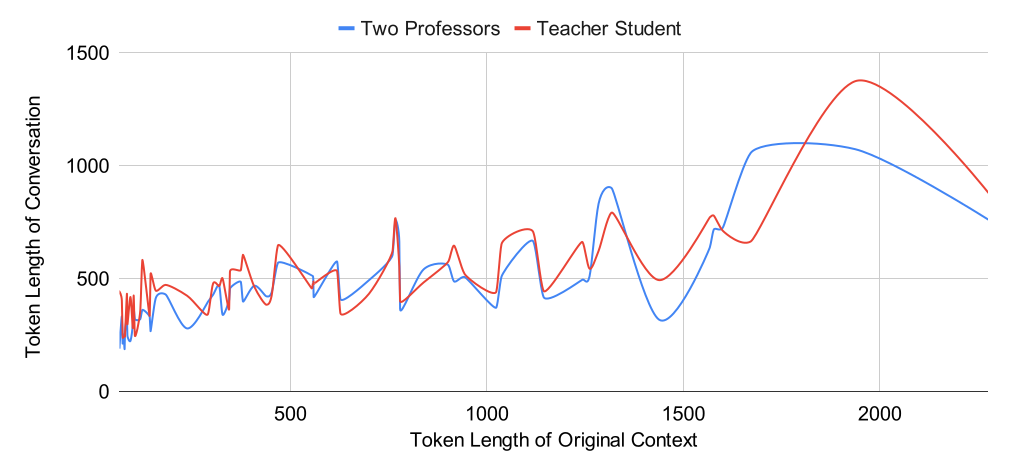
\includegraphics[width=0.8\columnwidth]{figures/context_len.pdf}
  \caption{With increasing context length the generated conversation length decreases!}
  \label{fig:context_length}
\end{figure}





Therefore, we conduct an experiment on 140k samples from the \owm corpus of varying input length to determine the optimal input token length that generates conversations of following characteristics: (1) retains all relevant information from the original context, (2) remains grounded to the source material and (3) enhances the conversation with complementary explanations and reasoning. For each sample, we generate conversations using two prompt (\tp and \ts) and observe the token length of the generations. As depicted in \autoref{fig:context_length}, with increasing input token length (X-axis), the token length of the generated conversation (Y-axis) does not scale up linearly. For example, an input context of 2K tokens results in a conversation that has 1K tokens resulting in a lot of information loss during conversion. Analyzing the \autoref{fig:context_length}, we see that the input token length of 500 can generate conversation that goes beyond 500 tokens meaning that the conversation not only retains information but also adds necessary reasoning  resulting in more tokens. 

% \begin{wrapfigure}{r}{0.5\textwidth}
%     \vspace{-6mm}
%     \centering    
%     \includesvg[width=\textwidth]{figures/context_len.svg}
%     \caption{With increasing context length the generated conversation length decreases!}
%   \label{fig:context_length}
%   % \vspace{-2mm}
% \end{wrapfigure}


\subsection{Conversation Length vs Model Performance}\label{ss:len_vs_acc}


As shown in \autoref{tab:7b_owm_4b}, \textsc{Longest Conversation} achieves the best results among all styles. Since \textsc{Longest Conversation} is curated by selecting the longest dialogue (in terms of token count) from seven conversations for a single context, it raises the question of how dialogue length impacts downstream task accuracy.

\begin{wraptable}[11]{r}{0.5\textwidth}
\centering
\vspace{-6mm}
\resizebox{\textwidth}{!}{% 
\begin{tabular}{@{}lcc@{}}
\toprule
\textbf{Style} &	\textbf{Avg Token Length} &	\textbf{Accuracy (Avg-All)}\\\toprule
\tp &  451.95	& 29.12 \\ 
\tss & 452.17	& 32.65 \\
\ps & 465.29	& 33.38 \\
\ts & 494.03 & 32.87 \\
\intr & 497.21	& 32.12 \\
\deb & 511.90	& 33.11 \\
\lk & 630.23	& 31.74 \\
\textsc{Longest Conversation} & 653.48	& 34.08\\
\toprule
\end{tabular}
}
\caption{\textbf{Conversation Length vs Downstream Task Accuracy:} Conversation length is not correlated with downstream task accuracy.}
\label{tab:len_vs_acc}
\end{wraptable} 

To explore the relationship between dialogue length and accuracy, we measured the average token length of dialogues across all conversational styles, including \textsc{Longest Conversation}. As seen in \autoref{tab:len_vs_acc}, reasoning accuracy does not exhibit a linear correlation with dialogue length. For example, with \ps style we can achieve comparable accuracy to \textsc{Longest Conversation} even when the average token length for \ps is \~ 188 lower than \textsc{Longest Conversation}. This highlights that the conversation length is not the only important factor to attain the maximum gain in reasoning ability. As mentioned in Section \ref{sec:ablations}, the structure and dynamics of the conversations also play a crucial role in maximizing reasoning gains.%The way conversations have been carried out is equally important.




\subsection{Conversation Quality Assessment}\label{ss:quality_assess}


% \paragraph{Conversation Quality Assessment.} \label{ss:quality_assess}
While the conversations generated by the \llm typically appear coherent, there are instances where the conversation fails to preserve the context or lacks grounding to the source material. In some cases, conversations may even be incomplete. Detecting poor-quality generation becomes challenging at scale. To address this, we explore two quality-filtering approaches:

\textbf{Heuristic Filtering.} We employ a simple heuristic based on token length. Given that the input context is limited to a maximum of 500 tokens and split into subcontexts of 500 tokens each to maximize information retention, we discard any generated conversations that fall below 50 tokens. This ensures that minimal information loss is detected early.

\textbf{\llm-based Scoring.} For a more comprehensive assessment, we use an \llm to score the quality of the generated conversations. We introduce four key metrics for evaluation:
\begin{itemize}[leftmargin=*] 
    \item \textbf{Correctness}: Verifies that all information, such as numbers and parameters, is accurately reflected in the conversation.
    \item \textbf{Faithfulness}: Ensures the conversation remains grounded in the context provided.
    \item \textbf{Information Preservation}: Checks whether all relevant facts and knowledge from the original context are retained in the conversation.
    \item \textbf{New Knowledge}: Evaluates whether the conversation introduces additional explanations, reasoning, or definitions not present in the raw input.
\end{itemize}




% \begin{figure}[H]
%   \centering
%   \includesvg[width=0.8\columnwidth]{figures/quality.svg}
%   \caption{LLM tends to rate its generation higher most of the times.}
%   \label{fig:conv_quality}
% \end{figure}


Given a raw context and its corresponding conversation, we ask $\mathcal{M}$ to rate the conversation on a scale of 1 to 5 in each of four metrics, with 1 representing poor quality and 5 representing the best possible conversation. To determine the overall quality, we compute the average score across the metrics and choose conversations with average scores more than or equal to 3. Additionally, we utilize the prompt from the FineWebEdu \citep{penedo2024finewebdatasetsdecantingweb} annotation framework to further check the correlation between two scoring approaches. In \autoref{fig:conv_quality}, we plot the scores for 140K conversations using FineWebEdu metrics and our metrics. It is clearly visible from the figure is that \llm tends to rate its own generation higher almost all the time resulting in a skewed distribution of rating. Around 96\% of conversations are labelled as high quality. However, compared to FineWebEdu, our metric results in less skewed distribution---making our approach more suitable for evaluating synthetic data derived from a seed corpus. % comparison between fineweb metrics and our. our is better

\begin{wrapfigure}{r}{0.5\textwidth}
    % \vspace{-6mm}
    \centering    
    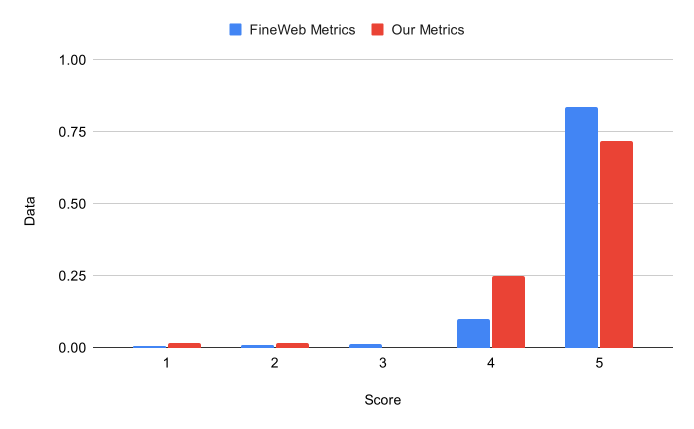
\includegraphics[width=\textwidth]{figures/quality.pdf}
    \caption{LLM tends to rate its generation higher most of the times.}
  \label{fig:conv_quality}
  % \vspace{-2mm}
\end{wrapfigure}

To further investigate, we choose 20 contexts and their corresponding conversations and manually label them on the above four metrics. We later pass these samples to \llm to obtain the quality scores. The correctness and faithfulness metrics were consistently high, with \llm showing a generation correct 96\% of times and human annotators labeling a conversation correct 98\% of times (with spearman correlation between two being 0.82) which validates the quality and reliability of the generated synthetic dialogues.  When comparing the overall human scores with those from the \llm across the four metrics, we observe a weak correlation between two sets (Spearman's $\rho=0.03$) and the reasoning behind them. Human annotators prioritized the information preservation metric, while the \llm often overlooked minor information loss. Additionally, the interpretation of ``New Knowledge" differed between humans and the \llm. Humans valued extra reasoning and explanation as forms of new knowledge, whereas the \llm assigned higher ``New Knowledge" scores to conversations containing out-of-context information that is difficult to verify. Given these differences in the results from human and \llm-based quality filtering, we use simple heuristic filtering in this study and plan to explore other approaches in the future.

\subsection{Compare with \dsm}\label{ss:dsm}

To asses the quality of our data, we run pre-training experiments to compare \ourdata with the recently released \dsm \citep{deepseek-math}. The \dsm approach is iterative. They construct a dataset for binary classification consisting of 500K positive data points randomly sampled from \owm (the seed corpus) and 500K negative data points randomly sampled from \cc. They train a fastText \citep{joulin2016fasttext} classifier on these data which they then use to extract samples from \cc as math content. All \cc domains for which over 10\% of the existing web pages have been extracted are at this point understood to be math-related. URLs which are associated with these domains but which have yet to be collected are manually labeled as math content. The web pages hosted at these addresses are added to the seed corpus and the classifier is retrained. \dsm performs 4 rounds in total resulting in the \dsm Corpus, consisting of some 120B math tokens. They continuously train a partially converged 7B \textsc{DeepSeekCoder-v1.5} model on a 500B token blend to attain the \dsm model and achieve substantial improvement on several math tasks. In contrast, \ourapproach proposes a simple alternative for generating high-quality math data that boosts the mathematical reasoning ability of \llm given access to a small seed corpus. 

As the \dsm dataset is not public, we replicate our previous blend, $\mathcal{D} = \{\mathcal{X}\cup \mathcal{R}_{pt}\}$, where $\mathcal{X} = \{\text{\ourdata-4B} \text{ (conversations of all styles except the \tss one)} \cup \text{\ourdata-14B (\tss conversations)}\}$. We maintain a 2:1 ratio of $\mathcal{X}$ and $\mathcal{R}_{pt}$ in the training blend. Similar to the approach of \dsm, we take a converged \textsc{DeepSeekCoder-v1.5} model as $\mathcal{C}$ --- the unconverged model weights are unpublished as far as we are aware --- and convert the model weights to a format compatible with Megatron-LM, which serves as our training framework, before continuously training for 500B tokens. We use a cosine learning rate schedule with a 19B token linear ramp-up, a maximum learning rate of 3e-4, and a minimum learning rate of 3e-6, and we anneal the learning rate over 500B tokens. We use Adam with parameters $\beta_{1}=0.9$ and $\beta_{2}=0.95$, a weight decay of 0.1, a gradient clipping threshold of 1.0, a sequence length of 4096, and a global batch size of 2304 sequences.

\begin{table*}[ht!]
\begin{center}
\resizebox{\textwidth}{!}{% 
\begin{tabular}{@{}lcccccccc@{}}
\toprule
\textbf{Dataset} & \textbf{Tokens} & \textbf{GSM8K} &\textbf{MATH} & \textbf{\shortstack{MMLU-\\STEM}} & \textbf{MMLU}& 	\textbf{\shortstack{\textsc{General Reasoning}\\(Avg)}} & \textbf{Avg-Math} & \textbf{Avg-All}\\\toprule
\dsm \citep{deepseek-math}& \multirow{3}{*}{500B} & 59.29	& 4.37	& 55.41	& 54.98	& 55.94 & 39.69 & 43.64\\ \cmidrule{3-9}
\ourdata-4B/14B [Combinations$^*$] & & 57.32 &	2.36	&51.95&	56.54	&59.16	& 37.21 &43.84\\ 
% \ourdata-14B [All Conversations] & & 52.46 &	3.24	&54.96&	59.20	&59.38	& 43.57\\ 
\toprule
\end{tabular}
}
\end{center}
\caption{\textbf{\dsm vs All Synthetic Conversations.} A model trained on conversations generated by \ourapproach from a small seed corpus can achieve math accuracy comparable to the \dsm model trained on 120B unique tokens.}
\label{tab:dsm_exp}
\end{table*}

From \autoref{tab:dsm_exp}, we can see that a model trained on conversations which \ourapproach generated given a small seed corpus can attain math accuracies comparable to the \dsm model with access to 120B unique math tokens in its continuous training blend. In fact, we outperform \dsm in \mmlu and general reasoning tasks, reaching higher average accuracy across all tasks. This underscores the quality of \ourapproach generated conversations and signifies the efficacy of \ourapproach in improving mathematical reasoning ability of \llm when the underlying raw data is limited.



In contrast to our prior $\mathcal{C}$, \dsm-7B \llm is a strong math baseline that has been specifically designed for addressing mathematical reasoning ability and surpasses \cite{azerbayev2023llemma}, \cite{gemmateam2024gemmaopenmodelsbased}, \cite{jiang2023mistral7b}, \cite{lewkowycz2022solvingquantitativereasoningproblems}, \cite{javaheripi2023phi}, \cite{dubey2024llama} [8B] base models on diverse math tasks. To evaluate the effectiveness of \ourapproach with stronger pretrained model, we perform an additional experiment, similar to our training setup in Section \ref{ss:training_details} using $\mathcal{C}=$ \dsm-7B. Specifically, we have continuously trained the $\mathcal{C}$ on 500B tokens maintaining a 2:1 ratio of math ($\mathcal{R}$) and 13 CC ($\mathcal{R}_{pt}$) dataset where the total blend is $\mathcal{D} = \{\mathcal{R}\cup \mathcal{R}_{pt}\}$. We conduct two experiments by alternating $\mathcal{R}$ with raw (\owma-14B) and $\mathcal{X}$.

\begin{table*}[ht!]
\begin{center}
\resizebox{\textwidth}{!}{% 
\begin{tabular}{@{}lcccccccc@{}}
\toprule
\textbf{Dataset} & \textbf{Tokens} & \textbf{GSM8K} &\textbf{MATH} & \textbf{\shortstack{MMLU-\\STEM}} & \textbf{MMLU}& 	\textbf{\shortstack{\textsc{General Reasoning}\\(Avg)}} & \textbf{Avg-Math} & \textbf{Avg-All}\\\toprule
\owma-14B & \multirow{3}{*}{500B} & 39.42	& 1.59	& 49.92	& 52.87	& 55.47 & 30.31 & 37.34\\ \cmidrule{3-9}
\ourdata [\textsc{all conversations}] & & 57.32 &	2.36	&51.95&	56.54	&59.16	& 37.21 &43.84\\ 

\toprule
\end{tabular}
}
\end{center}
\caption{\textbf{Training \dsm-7B with Raw Data vs All Synthetic Dialogues.} A strong pretrained \llm continously trained on conversations generated by \ourapproach provides significant boost in math accuracy than the same model trained on raw data---showing the effectiveness of \ourapproach regardless of pretraining model quality.}
\label{tab:dsm_exp_comp}
\end{table*}

As shown in \autoref{tab:dsm_exp_comp}, model trained on \ourdata data shows consistent improvement over model trained on raw data---resulting in 17.90\% gain on \gsm, 6.90\% average improvement across math tasks and 3.43\% average improvement across ten general reasoning tasks. These results further solidifies the effectiveness of \ourapproach regardless of the quality of the pretrained model. 



\subsection{Conversations on Code Tasks}\label{ss:code}



Unlike raw data, conversations tend to break down the context into sub-context and participants exchange their reasoning about the sub-context in a single turn. This feature is particularly useful for mathematical or logical reasoning which require step-by-step reasoning. However, this structure might hurt performance of \llm in domains where sequence of context needs to be preserved such as in codes. To further investigate the impact of conversational data on the coding capabilities of \llm, we conduct an evaluation of models trained on both raw and synthetic data across four established coding benchmarks: HumanEval \citep{chen2021evaluating}, MBPP \citep{austin2021program}, HumanEval+, and MBPP+ \citep{liu2024your}. These benchmarks are specifically designed to assess the model's ability to generate functional code in response to given prompts.


Our results, as presented in \autoref{tab:7b_code}, demonstrate that conversational synthetic data does not enhance coding performance. This is largely due to the way conversations tend to fragment code, wrapping it in natural language and thereby obscuring the intended sequence and logic inherent in programming tasks. Consequently, while conversations may be effective in contexts that benefit from collaborative reasoning, they are not suited for preserving the integrity of code, leading to diminished performance in coding benchmarks. 


\begin{table*}[ht]
\begin{center}
\resizebox{\textwidth}{!}{% 
\begin{tabular}{@{}lcccccc@{}}
\toprule
\textbf{Dataset} & \textbf{Style} & \textbf{HumanEval}        & \textbf{HumanEval+} & \textbf{MBPP (Sanitized)} & \textbf{MBPP+} & \textbf{Avg-All}\\\toprule
\owma-4B &   Raw & 12.20	& 10.98&	23.74 &0.00	&11.73 \\\midrule
Rephrase-\owma-4B & Rephrase &5.49	& 4.27	&20.23	&0.53	&7.63\\\midrule
% & \mawps           & \textbf{69.83}         & 66.83            \\ 
\multirow{9}{*}{\ourdata-4B} %& \textsc{Rephrase} & 5.49	& 4.27	&20.23	&0.53	&7.63\\\cmidrule{2-7}
& \tp & 8.54	& 4.88	&20.62	&0.00	    &8.51\\ 
 & \ts & 13.41	& 9.76	&26.46	&0.26	&12.47\\ 
& \tss & 10.37	& 7.93	&26.07	&0.26	&11.16\\  
& \lk & 10.37	& 8.54	&26.46	&0.79	&11.54\\
& \deb & 11.59	& 9.15	&24.90	&0.26	&11.48\\
& \intr & 7.32	& 4.88	&23.35	&0.26	&8.95\\
& \ps & 9.76	& 9.15	&24.51	&0.26	&10.92\\ \cmidrule{2-7}
& \textsc{Longest Conversation} & 9.15	& 7.32	& 28.40	& 0.53	& 11.35\\
& \textsc{All Conversations} & 12.20	& 9.15	& 28.02	& 0.53	& 12.48\\ \midrule
\owma-4B+\ourdata-4B [1:1] & \multirow{2}{*}{Combination} & 13.41	& 10.98	& 23.35	& 0.00	& 11.94\\ 
\owma-4B+\ourdata-4B [Concat] & & 10.37	& 7.93	& 31.52	& 0.00	& 12.46\\
\toprule
\end{tabular}
}
\end{center}
\caption{\textbf{Results of 7B \llm on Code Tasks:} Conversations and rephrases are ineffective for code benchmarks.}
\label{tab:7b_code}
\end{table*}

Interestingly, we also observe that rephrasing, which resembles raw data more closely in structure, further degrades coding accuracy. Our qualitative analysis of the rephrased documents reveals that the conversation generator (\llama) often removes critical elements such as important tags and code indentation, which are essential for comprehending and executing code correctly. This finding underscores the necessity of designing code-specific prompts that retain the structural components vital for coding tasks. 


\clearpage
\section{Dialogue Examples}\label{ss:conv_example}

% \textbf{\textsc{Raw Text}}
% \begin{tcolorbox}[colback=blue!5!white,colframe=white]
% \# The Truth about Martin Luther King Jr
  
% By Murray Bourne, 09 Jul 2006

% While King's influence on the civil rights movement was overall a Good Thing, I found the King Papers Project interesting, considering he was quite a plagiariser.

% Stanford's own King Encyclopedia gives some background but there is no mention of plagiarism.

% Wikipedia has more on King's authorship issues.
% Was his plagiarism sloppy academic writing or dishonesty? 

% This is the dilemma we face every time we find that a student has copied...

% Footnote: There are some interesting comments on King at Myths of Martin Luther King. Both of these sites have questionable reliability, of course. You have been warned.

% See the 1 Comment below.

% \#\#\# One Comment on "The Truth about Martin Luther King Jr"
% 1. Vinod says:

% If I have seen further, it is by standing on the shoulders of giants.

% \#\#\# Comment Preview

% HTML: You can use simple tags like $<$b$>$, $<$a href=``...''$>$, etc.

% To enter math, you can can either:
% 1. Use simple calculator-like input in the following format (surround your math in backticks, or qq on tablet or phone):

% $a^2 = sqrt(b^2 + c^2)$

% (See more on ASCIIMath syntax); or

% 2. Use simple LaTeX in the following format. Surround your math with \$\$ and \$\$.

% $\$\$\int g dx = \sqrt{\frac{a}{b}}\$\$$

% (This is standard simple LaTeX.)

% NOTE: You can't mix both types of math entry in your comment.

% \end{tcolorbox}

\textbf{\textsc{Raw Text}}
\begin{tcolorbox}[colback=blue!5!white,colframe=white]
\# CAT Quantitative Aptitude Questions | CAT Ratios, Mixtures, Alligations and Averages Questions

\#\#\#\#\#\# CAT Questions | Mixtures and Alligations | Mixtures - Range

The question is from CAT Ratio, Mixtures and Averages. Given the details about two alloys, we need to determine the possible values the weight of an ally can take. CAT exam is known to test on basics rather than high funda ideas. A range of CAT questions can be asked from Ratios and Proportions, Mixtures, Alligations and Averages. Make sure you master the topics. 2IIMs CAT questions bank provides you with CAT questions that can help you gear for CAT Exam CAT 2020.

Question 16: 100 kgs of an alloy of tin and lead in the ratio 1:3 is mixed with x kgs of an alloy of tin and lead in the ratio 3:2. If the overall alloy should contain between 40\% and 50\% tin, what is the range of values x can take?

1. 100 kgs $\leq x \leq$ 200 kgs

2. 80 kgs $\leq x \leq$ 240 kgs

3. 110 kgs $\leq x \leq$ 220 kgs

4. 75 kgs $\leq x \leq$ 250 kgs

\#\# Best CAT Coaching in Chennai

\#\#\#\# CAT Coaching in Chennai - CAT 2020Online Batches Available Now!
\end{tcolorbox}

\vspace{6mm}

% \textbf{\textsc{Synthetic Dialogue [\tp]}}

% \begin{tcolorbox}[colback=red!5!white,colframe=white]
% \textbf{Professor 1:} You know, I was reading about Martin Luther King Jr. and I came across some interesting information. While his influence on the civil rights movement was undoubtedly a good thing, I found out that he was quite a plagiarizer.

% \textbf{Professor 2:} Really? I hadn't heard that about him. What's the source of this information?
% Professor 1: Well, I was looking at the King Papers Project, and it's quite revealing. Stanford's own King Encyclopedia doesn't mention it, but Wikipedia has more on King's authorship issues.

% \textbf{Professor 2:} That's fascinating. Do you think his plagiarism was just sloppy academic writing or outright dishonesty?

% \textbf{Professor 1:} Exactly! That's the dilemma we face every time we find that a student has copied. It's hard to know whether it's just laziness or intentional deception.

% \textbf{Professor 2:} I see what you mean. By the way, I love that quote from Isaac Newton: "If I have seen further, it is by standing on the shoulders of giants." It's a great reminder that we all build on the work of others.

% \textbf{Professor 1:} Ah, nice connection! And yes, it's a great quote. By the way, I also came across some interesting comments on King at Myths of Martin Luther King. Of course, one has to be cautious about the reliability of those sources, but still...

% \textbf{Professor 2:} Absolutely. We always need to approach these kinds of sources with a critical eye. Thanks for sharing this, it's definitely given me something to think about.
% \end{tcolorbox}

\textbf{\textsc{Synthetic Dialogue [\tp]}}

\begin{tcolorbox}[colback=red!5!white,colframe=white]
\textbf{Professor 1:} Good morning, colleague. I'd like to discuss a question from CAT Ratio, Mixtures, and Averages. It's about two alloys of tin and lead, and we need to determine the possible values of the weight of an alloy.

\textbf{Professor 2:} Ah, yes. I'm familiar with this type of question. It's a classic example of Mixtures and Alligations. Please go ahead and share the details of the question.

\textbf{Professor 1:} We have 100 kgs of an alloy of tin and lead in the ratio 1:3, which means it has 25 kgs of tin and 75 kgs of lead. This alloy is mixed with x kgs of another alloy of tin and lead in the ratio 3:2. The overall alloy should contain between 40\% and 50\% tin. We need to find the range of values x can take.

\textbf{Professor 2:} That's a great problem. We can start by analyzing the second alloy. If it has a ratio of 3:2, that means it has 3x/5 kgs of tin and 2x/5 kgs of lead, with a total weight of x kgs.

\textbf{Professor 1:} Exactly. Now, when we mix these two alloys, how does the mixture change? We need to find the overall percentage of tin in the resulting alloy.

\textbf{Professor 2:} Right. Let's think about it. If the overall alloy should contain between 40\% and 50\% tin, what does that imply about the range of values x can take?

\textbf{Professor 1:} That's the key question. If we can determine the range of x, we can answer the question. Do you think it's possible to narrow down the options to one of the given choices?

\textbf{Professor 2:} Yes, I think so. Let's analyze the options. We have 1. 100 kgs $\leq x \leq$ 200 kgs, 2. 80 kgs $\leq x \leq$ 240 kgs, 3. 110 kgs $\leq x \leq$ 220 kgs, and 4. 75 kgs $\leq x \leq 250$ kgs. Which one do you think is the correct answer?

\textbf{Professor 1:} Well, after analyzing the problem, I think the correct answer is option 2: 80 kgs $\leq x \leq$ 240 kgs. What do you think?

\textbf{Professor 2:} I agree with you. The correct answer is indeed option 2. Well done! This question is a great example of how CAT exam tests our understanding of basics rather than high-funda ideas.
\end{tcolorbox}


\clearpage

\textbf{\textsc{Raw Text}}
\begin{tcolorbox}[colback=blue!5!white,colframe=white]
?

Free Version

Moderate

\# Interpretation of Equilibrium from Graph of Concentration vs Time

CHEM-NWU9LE

Consider the graph below of a chemical reaction observing the concentration of two chemical species with time.

Which species is the reactant?
\$\$

Which species is the product?

\$\$

At what region does the solution appear to be in equilibrium?
\$\$

What is the $K_c$ for the reaction?
\end{tcolorbox}

\vspace{6mm}

\textbf{\textsc{Synthetic Dialogue [\ts]}}

\begin{tcolorbox}[colback=red!5!white,colframe=white]

\textbf{Student:} Hi, teacher. I'm having trouble understanding this graph of a chemical reaction. Can you help me?

\textbf{Teacher:} Of course! What's your first question about the graph?

\textbf{Student:} Okay, so which species is the reactant?

\textbf{Teacher:} Let's take a look at the graph. The species whose concentration is decreasing with time is the reactant. Can you identify which one that is?

\textbf{Student:} Ah, I think it's... (looks at the graph) ...the one whose concentration starts high and decreases.

\textbf{Teacher:} That's correct! The reactant is the species whose concentration starts high and decreases with time. Now, what's your next question?

\textbf{Student:} Which species is the product?

\textbf{Teacher:} Good question! The product is the species whose concentration starts low and increases with time. Can you identify which one that is?

\textbf{Student:} Yeah, I think it's... (looks at the graph) ...the one whose concentration starts low and increases.

\textbf{Teacher:} That's right! The product is the species whose concentration starts low and increases with time. Now, what's your next question?

\textbf{Student:} At what region does the solution appear to be in equilibrium?

\textbf{Teacher:} Look at the graph again. At what point does the concentration of both species seem to be constant, not changing with time?

\textbf{Student:} Hmm... I think it's... (looks at the graph) ...after a certain time, when the lines are flat.

\textbf{Teacher:} Exactly! The solution appears to be in equilibrium when the concentration of both species is constant, which is after a certain time when the lines are flat. Now, what's your next question?

\textbf{Student:} What is the Kc for the reaction?

\textbf{Teacher:} Unfortunately, the graph doesn't provide enough information to calculate the Kc value. We would need more data or information about the reaction to determine the equilibrium constant, Kc.

\textbf{Student:} Okay, I think I understand now. Thank you for your help!
\end{tcolorbox}

\clearpage

\textbf{\textsc{Raw Text}}
\begin{tcolorbox}[colback=blue!5!white,colframe=white]
    
    What's the probability that: The person is not age 18 to 34 and does not own an iPhone?
    
    The presidential election is coming.
    
    Five survey companies (A, B, C, D, and E) are doing survey to forecast whether or not the Republican candidate will win the election.
    
    Each company randomly selects a sample size between 1000 and 1500 people.
    
    All of these five companies interview people over the phone during Tuesday and Wednesday.
    
    The interviewee will be asked if he or she is 18 years old or above and U.S. citizen who are registered to vote. If yes, the interviewee will be further asked: will you vote for the Republican candidate?
    
    On Thursday morning, these five companies announce their survey sample and results at the same time on the newspapers.
    
    The results show that a\% (from A), b\% (from B), c\% (from C), d\% (from D), and e\% (from E) will support the Republican candidate.
    
    The margin of error is plus/minus 3\% for all results.
    
    Suppose that $c{>}{a}{>}{d}{>}{e}{>}{b}$.
    When you see these results from the newspapers, can you exactly identify which result(s) is (are) not reliable and not accurate?
    
    That is, can you identify which estimation interval(s) does (do) not include the true population proportion?
    
    If you can, explain why you can, if no, explain why you cannot and what information you need to identify.
    
    Discuss and explain your reasons. You must provide your statistical analysis and reasons.
\end{tcolorbox}

% \clearpage

\textbf{\textsc{Synthetic Dialogue [\tss]}}

\begin{tcolorbox}[enhanced jigsaw,breakable,pad at break*=1mm,colback=red!5!white,colframe=white]
\textbf{**Turn 1**}

Alex: Hey Ben, have you started working on our assignment about the presidential election survey?

Ben: Yeah, I've been going over the context. It seems like we need to identify which survey result is not reliable and accurate.

Alex: Exactly! Let's break it down. We have five survey companies, A, B, C, D, and E, each with a sample size between 1000 and 1500 people.

Ben: Right, and they all have a margin of error of plus/minus 3\%.



\textbf{**Turn 2**}

Alex: Okay, so we're given that c $>$ a $>$ d $>$ e $>$ b. What does this tell us?

Ben: It tells us the order of the proportions of people who will support the Republican candidate according to each survey company.

Alex: That's right. And since the margin of error is the same for all companies, we can assume that the true population proportion should lie within a similar range for all companies.



\textbf{**Turn 3**}

Ben: But wait, if the true population proportion lies within a similar range, then shouldn't all the estimation intervals overlap?

Alex: Exactly! If the estimation intervals don't overlap, it means that at least one of them is not reliable and accurate.

Ben: So, we need to check if the intervals overlap. How do we do that?



\textbf{**Turn 4**}

Alex: Let's calculate the estimation intervals for each company. For company A, it's a\% $\pm$ 3\%, and similarly for the others.

Ben: Okay, got it. So, we have a\% $\pm$ 3\%, b\% $\pm$ 3\%, c\% $\pm$ 3\%, d\% $\pm$ 3\%, and e\% $\pm$ 3\%.

Alex: Now, let's check if these intervals overlap. Since c $>$ a $>$ d $>$ e $>$ b, the interval for company C should be the highest, and the interval for company B should be the lowest.



\textbf{**Turn 5**}

Ben: I see what you're getting at. If the intervals overlap, then the highest value of the lowest interval (company B) should be greater than or equal to the lowest value of the highest interval (company C).

Alex: That's right! If that's not the case, then we know that at least one of the intervals is not reliable and accurate.

Ben: Let's plug in some numbers and see if we can identify which one is not reliable.



\textbf{**Turn 6**}

Alex: Alright, let's say the results are a = 45\%, b = 38\%, c = 50\%, d = 42\%, and e = 40\%. Can we identify which one is not reliable?

Ben: Let's calculate the estimation intervals... (calculates)...and check if they overlap.

Alex: (checks the calculations) Ah, look at that! The interval for company B (38\% $\pm$ 3\%) doesn't overlap with the interval for company C (50\% $\pm$ 3\%).

Ben: That means company B's result is not reliable and accurate!



\textbf{**Turn 7**}

Ben: But why can't we identify the other unreliable results, if any?

Alex: That's because we only have the relative order of the proportions, not the exact values. We need more information to identify other unreliable results, if any.

Ben: I see. So, we can only identify company B's result as not reliable and accurate, but we can't say for sure about the others.

Alex: That's correct. We've done our best with the given information.
\end{tcolorbox}

\clearpage


\textbf{\textsc{Raw Text}}
\begin{tcolorbox}[colback=blue!5!white,colframe=white]
  \# Decimal to Percent Calculator.
  
  The calculator will convert decimal into percent, with steps shown.
  
  If the calculator did not compute something or you have identified an error, or you have a suggestion/feedback, please write it in the comments below.
  
  Convert $1.4$ into decimal.  \#\# Solution From the converting decimal to percent note, we know that to obtain a percent, we need to multiply a decimal by $100$.
  
  But multiplying by $100$is equivalent to moving a decimal point $2$ positions to the right.
\end{tcolorbox}

\vspace{6mm}

\textbf{\textsc{Synthetic Dialogue [\lk]}}

\begin{tcolorbox}[colback=red!5!white,colframe=white]
    \textbf{**Turn 1**}
    
    Layman: Hi, I'm not sure what this calculator does. Can you explain it to me?
    
    Me: This calculator converts decimals into percents. It shows the steps to do the conversion.
    
    \textbf{**Turn 2**}
    
    Layman: Okay, got it. So what's the problem we're trying to solve?
    
    Me: We're trying to convert 1.4 into a percent.
    
    \textbf{**Turn 3**}
    
    Layman: How do we do that? Is there a formula or something?
    
    Me: Yes, there is. According to the note on converting decimal to percent, we need to multiply the decimal by 100 to obtain a percent.
    
    
    \textbf{**Turn 4**}
    
    Layman: Why do we need to multiply by 100? What's the logic behind it?
    
    Me: Well, I'm not sure about the logic, but the note says that's what we need to do. But I can tell you that multiplying by 100 is equivalent to moving the decimal point 2 positions to the right.
    
    \textbf{**Turn 5**}
    
    Layman: What do you mean by moving the decimal point 2 positions to the right? Can you explain that?
    
    Me: Sure. When you multiply a number by 100, the decimal point shifts 2 places to the right. For example, if you have 1.4 and you multiply it by 100, the decimal point will move 2 places to the right, making it 140.
    
    \textbf{**Turn 6**}
    
    Layman: Ah, I think I understand now. So, if we multiply 1.4 by 100, what do we get?
    
    Me: That's right! If we multiply 1.4 by 100, we get 140. And that's the equivalent percent value of the decimal 1.4.
\end{tcolorbox}

\clearpage


\textbf{\textsc{Raw Text}}
\begin{tcolorbox}[colback=blue!5!white,colframe=white]
Try to finish the derivation and see how it applies to the sum you're trying to compute. Sorry if this is hard to understand.

7. Jun 14, 2009

\#\#\# jgens

Cyosis, why would he/she use the sum for the first n natural numbers when his sum asks for odd natural numbers only?

8. Jun 14, 2009

\#\#\# Cyosis

If you know the sum for the first n natural numbers you can quickly solve the sum for the first odd numbers. Had he known it, it would have been the easiest way to calculate the sum he's interested in.

9. Jun 14, 2009

\#\#\# Manchot

The story is that a six-year-old Gauss was told by his teacher to add the numbers 1 to 100 as a form of busywork. In seconds, he came up with the answer, much to his teacher's surprise. What he did was notice that since 1+100=101, 2+99=101, 3+98=101, etc., the sum becomes a simple multiplication: there are 50 of the above \"pairs,\" so the sum is just 50*101 = 5050. Anyway, that's the intuition behind the identity that Cyosis posted. You can pretty much use the exact same intuition.

10. Jun 14, 2009

\#\#\# gabrielh

Okay thanks, I get it now.


11. Jun 14, 2009
\end{tcolorbox}

\vspace{6mm}


\textbf{\textsc{Synthetic Dialogue [\deb]}}

\begin{tcolorbox}[colback=red!5!white,colframe=white]
\textbf{jgens}: I don't understand why Cyosis suggested using the sum of the first n natural numbers to solve the problem. The original problem asks for the sum of the first odd natural numbers, not all natural numbers.

\textbf{Cyosis}: I see what jgens is saying, but I think my approach is still valid. If you know the sum of the first n natural numbers, you can easily derive the sum of the first odd natural numbers. It's actually the easiest way to calculate the sum.

\textbf{Manchot}: I think I can help clarify things. The story about Gauss adding numbers from 1 to 100 is relevant here. He noticed that 1+100=101, 2+99=101, and so on, which makes the sum a simple multiplication problem. There are 50 such pairs, so the sum is 50*101 = 5050. This is the intuition behind Cyosis' suggestion.

\textbf{jgens}L I see what Manchot is saying, but I'm still not convinced. How does this story about Gauss relate to the sum of odd natural numbers?

\textbf{Cyosis}: Well, jgens, the same intuition applies here. We can use a similar pairing method to calculate the sum of odd natural numbers. It's not a direct application, but the principle is the same.

\textbf{gabrielh}: I think I'm starting to get it now. So, we can use the sum of the first n natural numbers as a stepping stone to calculate the sum of the first odd natural numbers, and the Gauss story provides the intuition behind this approach.

\textbf{Manchot}: Exactly, gabrielh! That's the idea. By understanding the sum of the first n natural numbers, we can derive the sum of the first odd natural numbers using a similar method.

\textbf{Cyosis}: I'm glad we could clarify things. The key is to recognize that the sum of the first n natural numbers is a more general problem that can be used to solve the more specific problem of the sum of the first odd natural numbers.
\end{tcolorbox}

\clearpage

\textbf{\textsc{Raw Text}}
\begin{tcolorbox}[colback=blue!5!white,colframe=white]

The Cryptographic Lens

Shafi Goldwasser - Colloquium Lecture - POSTPONED!

Tuesday, 21.10.2014, 14:30

Room 337-8 Taub Bld.

...

ceClub: A Centralized \"Zero-Queue\" Network Architecture

Jonathan Perry (MIT, CSAIL)

Monday, 06.10.2014, 11:00

EE Meyer Building 861

Current datacenter networks inherit the principles that went into the design of the Internet, where packet transmission and path selection decisions are distributed among the endpoints and routers. Instead, we propose that each sender should delegate control—to a centralized arbiter—of when each packet should be transmitted and what path it should follow. Fastpass is a datacenter network architecture built using this principle. Fastpass incorporates two fast algorit...


Parameterized Automata Constructions and Their Applications

Ran Ben-Basat

Monday, 22.09.2014, 15:30

Taub 701

Parameterization is a useful tool for handling NP-hard problems in the real world. It aims to reduce the running times of algorithms for such problems, by confining the combinatorial explosion to some parameter k. As this parameter is often significantly smaller than the input size, it allows to develop practical algorithms for non-trivial classes of instances for these problems. In this talk we present a novel framework for developing parameterized algorithms, using construction...

Observing the Observers: Social Context Analysis Using Computer Vision

Meir Cohen

Wednesday, 10.09.2014, 12:00

Taub 601

It is quite common that multiple human observers attend to a single point of interest.

Mutual awareness activity (MAWA) refers to the dynamic of this social phenomena.

A peak of a MAWA is known as a mutual awareness event (MAWE) and can be interpreted as a \"buzz\" event, which draws the attention of many observers.

A preferred way to monitor those social phenomenon is with a camera that captures the human observers while they observe the activity in the scene.

Our work studies the ...
\end{tcolorbox}

\vspace{6mm}

\textbf{\textsc{Synthetic Dialogue [\intr]}}

\begin{tcolorbox}[enhanced jigsaw,breakable,pad at break*=1mm, colback=red!5!white,colframe=white]

\textbf{Subject Matter Expert:} Unfortunately, the lecture was postponed, so we don't have any information about the specific topic she was going to cover. However, the title of the lecture was \"The Cryptographic Lens,\" which suggests that it might have been related to cryptography and its applications.

\textbf{Interviewer:} That's a shame it was postponed. Moving on, let's talk about the ceClub lecture by Jonathan Perry from MIT, CSAIL. Can you summarize the main idea behind his proposed datacenter network architecture, Fastpass?


\textbf{Subject Matter Expert:} Yes, certainly. Jonathan Perry proposed a centralized \"zero-queue\" network architecture called Fastpass, which is a departure from the traditional distributed approach used in Internet design. In Fastpass, each sender delegates control to a centralized arbiter, which decides when each packet should be transmitted and what path it should follow. This approach aims to improve the efficiency of datacenter networks.

\textbf{Interviewer:} That's fascinating. What can you tell me about the talk by Ran Ben-Basat on parameterized automata constructions and their applications?


\textbf{Subject Matter Expert:} Ran Ben-Basat discussed the concept of parameterization, which is a useful tool for handling NP-hard problems in the real world. The idea is to reduce the running times of algorithms for these problems by confining the combinatorial explosion to some parameter k. He presented a novel framework for developing parameterized algorithms using construction-based methods.


\textbf{Interviewer:} I see. Now, let's switch gears and talk about the lecture by Meir Cohen on social context analysis using computer vision. Can you explain what mutual awareness activity (MAWA) and mutual awareness event (MAWE) refer to in this context?


\textbf{Subject Matter Expert:} Yes. Mutual awareness activity (MAWA) refers to the dynamic of multiple human observers attending to a single point of interest. A peak of this activity is known as a mutual awareness event (MAWE), which can be interpreted as a \"buzz\" event that draws the attention of many observers. Meir Cohen's work focuses on monitoring and analyzing these social phenomena using computer vision, specifically by capturing the human observers with a camera while they observe the activity in the scene.

\end{tcolorbox}


\clearpage

\textbf{\textsc{Raw Text}}
\begin{tcolorbox}[colback=blue!5!white,colframe=white]
Note: At section X = 12 m, the speed is close to 1.5 m / s Thus for a return trip of 2x20m = 40 m to return to the profile X = 14m, the wave takes 27 s. Thus, the graph of Figure. 11 is located before the (eventual) reflected wave coming from the absorbing upstream boundary, which can disturb the sensors.

\#\# Comparative analysis of records

We have exploited some of the tests in a transversal manner, to identify particular behaviors of the surface waves:

• impact of the variation of the amplitude for several tests characterized by the same parameters but with roughnesses, or geometries either uniform, or linear

• impact of the change in the period

• impact of the variation of the initial amplitude

• comparison for the same test carried out in uniform or converging section

• impact of roughness variation


\#\#\# Impact of the variation of the amplitude for several tests with the same parameters

We have compared several tests characterized by D70, by Ab absorbing boundary conditions and for the same period T5. These are tests D70A5T5, D70A2T2 and D70A5T7 in RoAbUn, SmAbCo and SmAbUn conditions

Figure 16 Figure 17 Figure 18

• Figure 16: amplitudes variations for the 3 runs are increasing according to the slope, which is in accordance with the theory.

• Figure 17: the initial amplitudes of the waves generated by the wave maker are not always well respected: all the curves of the same diagram should start from the same point to X = 0

• Figure 18: there is a sharp change in amplitude at the arrival at the top of the slope.
\end{tcolorbox}


% \vspace{6mm}

\textbf{\textsc{Synthetic Dialogue [\ps]}}

\begin{tcolorbox}[colback=red!5!white,colframe=white]

\textbf{User:} Hi, I'm analyzing some data on surface waves and I'd like to discuss some observations with you. Can you help me understand the impact of varying amplitude on surface waves?

\textbf{AI Assistant:} I'd be happy to help. From the context, I see that you have several tests with the same parameters but different amplitudes. Specifically, you have tests D70A5T5, D70A2T2, and D70A5T7 in RoAbUn, SmAbCo, and SmAbUn conditions. What would you like to know about these tests?

\textbf{User:} Yes, that's correct. I'm looking at Figures 16, 17, and 18. Can you explain what's happening in Figure 16?

\textbf{AI Assistant:} In Figure 16, the amplitudes of the waves are increasing according to the slope, which is consistent with theoretical expectations. This suggests that the amplitude of the wave is directly related to the slope of the surface.

\textbf{User:} That makes sense. But what about Figure 17? The initial amplitudes of the waves generated by the wave maker don't seem to be consistent.

\textbf{AI Assistant:} That's a good observation. Yes, the initial amplitudes of the waves don't start from the same point at X = 0, which is unexpected. This could be an issue with the wave maker or the experimental setup.

\textbf{User:} Okay, got it. And what about Figure 18? There seems to be a sudden change in amplitude at the top of the slope.

\textbf{AI Assistant:} Yes, that's correct. Figure 18 shows a sharp change in amplitude at the arrival at the top of the slope. This could be due to the interaction between the wave and the slope, causing a sudden increase or decrease in amplitude.

\textbf{User:} That's helpful. So, what can we conclude about the impact of varying amplitude on surface waves?

\textbf{AI Assistant:} Based on these figures, it seems that the amplitude of the wave is directly related to the slope of the surface, and changes in amplitude can affect the behavior of the wave. However, we also need to consider the potential issues with the wave maker or experimental setup that may be affecting the results.

\textbf{User:} Okay, that's a good summary. Thanks for your help in analyzing these figures!

\end{tcolorbox}


% \subsection{Continuous Training of Model with Larger Token Budget}

\end{document}
